\documentclass{article}

\usepackage{amsmath}
\usepackage{amsthm}
\usepackage{amssymb}
\usepackage{hyperref,enumitem,tcolorbox}
\usepackage{fancyhdr, bookmark, parskip}
\usepackage[hmarginratio=1:1]{geometry}
\setlength{\headheight}{28pt}
\newcommand{\R}{\mathbb{R}}
\newcommand{\C}{\mathbb{C}}
\newcommand{\Q}{\mathbb{Q}}
\newcommand{\Z}{\mathbb{Z}}
\newcommand{\F}{\mathbb{F}}
\newcommand{\N}{\mathbb{N}}
\usepackage{tcolorbox}
\usepackage{graphicx}
\newtheorem{thm}{Theorem}[section]
\newtheorem{prop}{Proposition}[section]
\newtheorem{cor}{Corollary}[thm]
\newtheorem{lem}{Lemma}[section]
\theoremstyle{definition}
\newtheorem{defn}{Definition}[section]
\newtheorem*{rem}{Remark}
\newtheorem*{ex}{Example}
\renewcommand\qedsymbol{$\blacksquare$}




\include{graphicsx}
\title{Solutions}
\author{Lance Remigio}

\begin{document}
\maketitle   

\begin{enumerate}
    \item \( x^{10} \cdot x^{11} = x^{10+11} = x^{21}\).
    \item \( \frac{y^4}{y^7} = \frac{1}{y^3} = y^{-3}.\)
    \item \( (2x^3)^4 = (2)^4 (x^3)^4 = 16x^{12}\).
    \item \( \sqrt{12} = \sqrt{ 4 \cdot 3 } = \sqrt{4} \sqrt{3} = 2 \sqrt{3}.\)
    \item \( |-12 \div -2| = \Big| \frac{-12}{-2} \Big| = | 6 | = 6.\)
    \item Following pemdas, we have 
        \begin{align*}
            \frac{6 + 50 - 4^2 }{100 \div (5 + 2^2 \times 5 )}&= \frac{40}{ \frac{100}{25}} \\
                                                              &= \frac{40}{4} \\
                                                              &= 10.
        \end{align*}
    \item Via distribution, we can write 
    \begin{align*}
        y(z+7) - 2z(y-6) &= yz+7y - 2zy + 12z \\
    \end{align*}
\item \[ (4x^2)(9y)(2xy) = 72x^3y^2.\]
\item Simplifying we get
    \begin{align*}
        \frac{12gk^6 n^4}{42 g^3 k^5 n }&= \frac{2kn^3}{7g^2} = \frac{2}{7}kn^3g^{-2}. \\
    \end{align*}
\item Simplifying we get 
\begin{align*}
    \frac{6a^{-5}b^4 d^{-1}}{8a^{-3}b^{-2}c^{-2}} &= \frac{6}{8} (a^{-5 - 3} \cdot b^{4 - 2 }) \cdot (d^{-1} \cdot c^{-2}) \\
                                                  &= \frac{6}{8} (a^{-8} \cdot b^2 \cdot d^{-1} \cdot c^{-2}) \\ 
                                                  &= \frac{6b^2}{8da^8c^2 }.
\end{align*}
\item If \( a = 3, b = -2, \)and \( c = 1/3\), then 
    \begin{align*}
        12c^2 + 2a(-3b - 1)&= 12(1/3)^2 + 2\cdot3(-3(-2) - 1 ) \\ 
                           &= \frac{12}{9} + 6(6-1) \\ 
                           &= \frac{12}{9} + 30 \\ 
                           &= \frac{12 + 30 \cdot 9 }{9} \\
                           &= \frac{12 + 270}{9} \\
                           &= \frac{282}{9} \\
                           &= 31\frac{1}{3}  \tag{\(\Leftarrow\) mixed fraction!}
    \end{align*} 
\item Multiplying we get \[ (x+4)(x-7) = x^2 + 4x - 7x -28 = x^2 -3x -28.\]
\item Observe that \[ (3x-5)(4x+2) = 12x^2 -20x + 6x -10 = 12x^2 -14x - 10.\]

    We can further simplify by factoring \(2\)  
    \[ 12x^2 -14x - 10 = 2(6x^2 - 7x - 5).\]
\item Observe that 
    \begin{align*}
        (y^2 - 4y + 2 )(y-3) &= y^3 -4y^2 +2y -3y^2 +12y - 6  \\
                             &= y^3 -7y^2 +14y - 6.
    \end{align*}
    Hence, 
    \[ (y^2 - 4y + 2 )(y-3) = y^3 -7y^2 +14y - 6.\]

\item What is the \textbf{Greatest Common Factor (GCF)} of \( 16x^2y^3\) and \(20x^3y\)?
    \begin{proof}[Solution]
        The \textbf{Greatest Common Factor} is \( \text{GCF}(16x^2y^3, 20x^3y) = 4x^2y\)
    \end{proof}
\item What is the \textbf{Least Common Multiple (LCM)} of \( 6x^2y\) and \( 8x^2y\)?
    \begin{proof}[Solution]
        The \textbf{Least Common Multiple (LCM)} is
        \[ \text{LCM}(6x^2y, 8x^2y) = \frac{|6x^2y \cdot 8x^2y|}{\text{GCF}(16x^2y^3, 20x^3y)} = \frac{6x^2y \cdot 8x^2y}{4x^2y} = 12 x^2 y .\]
    \end{proof}

Simplify. Assume all variables are positive.

\item \( \sqrt{75} + \sqrt{48}. \) 

    \begin{proof}[Solution]
    We can express \(75\) and \(28\) in terms of their prime factorizations. Hence, \( 75 = 5^2 \cdot 3 \) and \( 48 = 4^2 \cdot 3\). Therefore, we can write 
    \begin{align*}
        \sqrt{75} + \sqrt{48} &= \sqrt{5^2 \cdot 3 } + \sqrt{4^2 \cdot 3 } \\
                              &= (5 + 4)\sqrt{3} \\
                              &= 9 \sqrt{3}.
    \end{align*}
    Hence, 
    \[ \sqrt{75} + \sqrt{48} = 9 \sqrt{3}. \]
    \end{proof}
\item \( \sqrt{25a^2b^5}.\)

    \begin{proof}[Solution]
    Using our square root properties, we have 
    \begin{align*}
        \sqrt{25 a^2 b^5 }&= 5ab^{5/2}. \\
    \end{align*}
\end{proof}
\item \( \sqrt{14} \cdot \sqrt{2}.\)
\begin{proof}[Solution]
    Observe that 
    \begin{align*}
        \sqrt{14} \cdot \sqrt{2} &= \sqrt{2 \cdot 7} \cdot \sqrt{2} \\
    &= \sqrt{2} \cdot \sqrt{2} \cdot \sqrt{7} \\
    &= 2 \sqrt{7}.
    \end{align*}
\end{proof}

\item \( (x^6)^{1/2}\).
\begin{proof}[Solution]
    \( (x^6)^{1/2} = x^{6/2} = x^3.\)
\end{proof}

Solve the following equations.

\item \( 3k - 18 = -9k + 30 \).
\begin{proof}[Solution]
    Solving for \( k \), we write 
    \begin{align*}
        3k - 18 &= -9k + 30 \\
        \implies 12k &= 48 \\
        \implies k &= \frac{48}{12} \\ 
        \implies k &= 4.
    \end{align*}
\end{proof}

\item \( x^2 = 81\).
\begin{proof}[Solution]
    Solving for \(x \) by taking the square root, we get \( x = \pm \sqrt{81} = \pm 9.  \)
\end{proof}

\item \( -5 (2x - 1) = 15\).
\begin{proof}[Solution]
    Suppose \( -5(2x - 1) = 15\). Solving for \( x \), we get 
    \begin{align*}
        -5(2x-1)&= 15 \\
        -10x +5 &= 15 \\
        -10x &= 10 \\
        x &= -1.
    \end{align*}
\end{proof}

\item \( |-2x+5| = 7 \).
\begin{proof}[Solution]
    By definition of \( |\cdot|\), we have 
    \begin{align*}
        |-2x + 5 |&= 7  \\
        -2x + 5 &= \pm 7. 
    \end{align*}
Here we have two cases, either \( -2x + 5 = 7 \) or \( -2x + 5 = -7\). If \( -2x + 5 = 7 \), then 
we have 
\[ -2x + 5 = 7 \implies x = \frac{7-5}{-2} = -\frac{2}{2} = -1. \]
If \( -2x + 5 = -7 \), then we have 
\[ -2x + 5 = -7 \implies x = \frac{-7 - 5}{-2} = \frac{-12}{-2} = 6.\]
\end{proof}

\item Find the value of the variable
    \[ \frac{5}{7} = \frac{H}{6}.\]
\begin{proof}[Solution]
We have 
\begin{align*}
    \frac{5}{7} &= \frac{H}{6}  \\
     7H &= 30  \\
     \implies H &= \frac{30}{7}. \\
\end{align*}
\end{proof}

Use the following expressions to answer the questions below. 
\[ 3x ~~~~ 5-2ab ~~~~ 7z^2 + 6xyz - 9 ~~~~ 2x^2 -3x^5 +1 ~~~~ x^4.\]
\item Which expressions above are \textit{monomials}? 
    \begin{proof}[Solution]
    \( 3x \) and \( x^4 \) are \textit{monomials}.
    \end{proof}
\item Which expressions above are \textit{binomials}?  
    \begin{proof}[Solution]
    Only \( 5 - 2ab \) is a  \textit{binomial}.
    \end{proof}
\item Determine the polynomial with the highest degree. Write it in standard form and determine the degree and leading coefficient. 
    \begin{proof}[Solution]
    The polynomial with the highest degree is \( 2x^2 -3x^5 +1\) which is a 5th degree polynomial and its standard form is \( -3x^5 +2x^2 + 1 \) with a leading coefficient of \(-3\).  
    \end{proof}

\item Graph the equation \( y = 2x - 5 \).
    \begin{proof}[Solution]
    Graphing the equation above looks like
    \begin{center}
        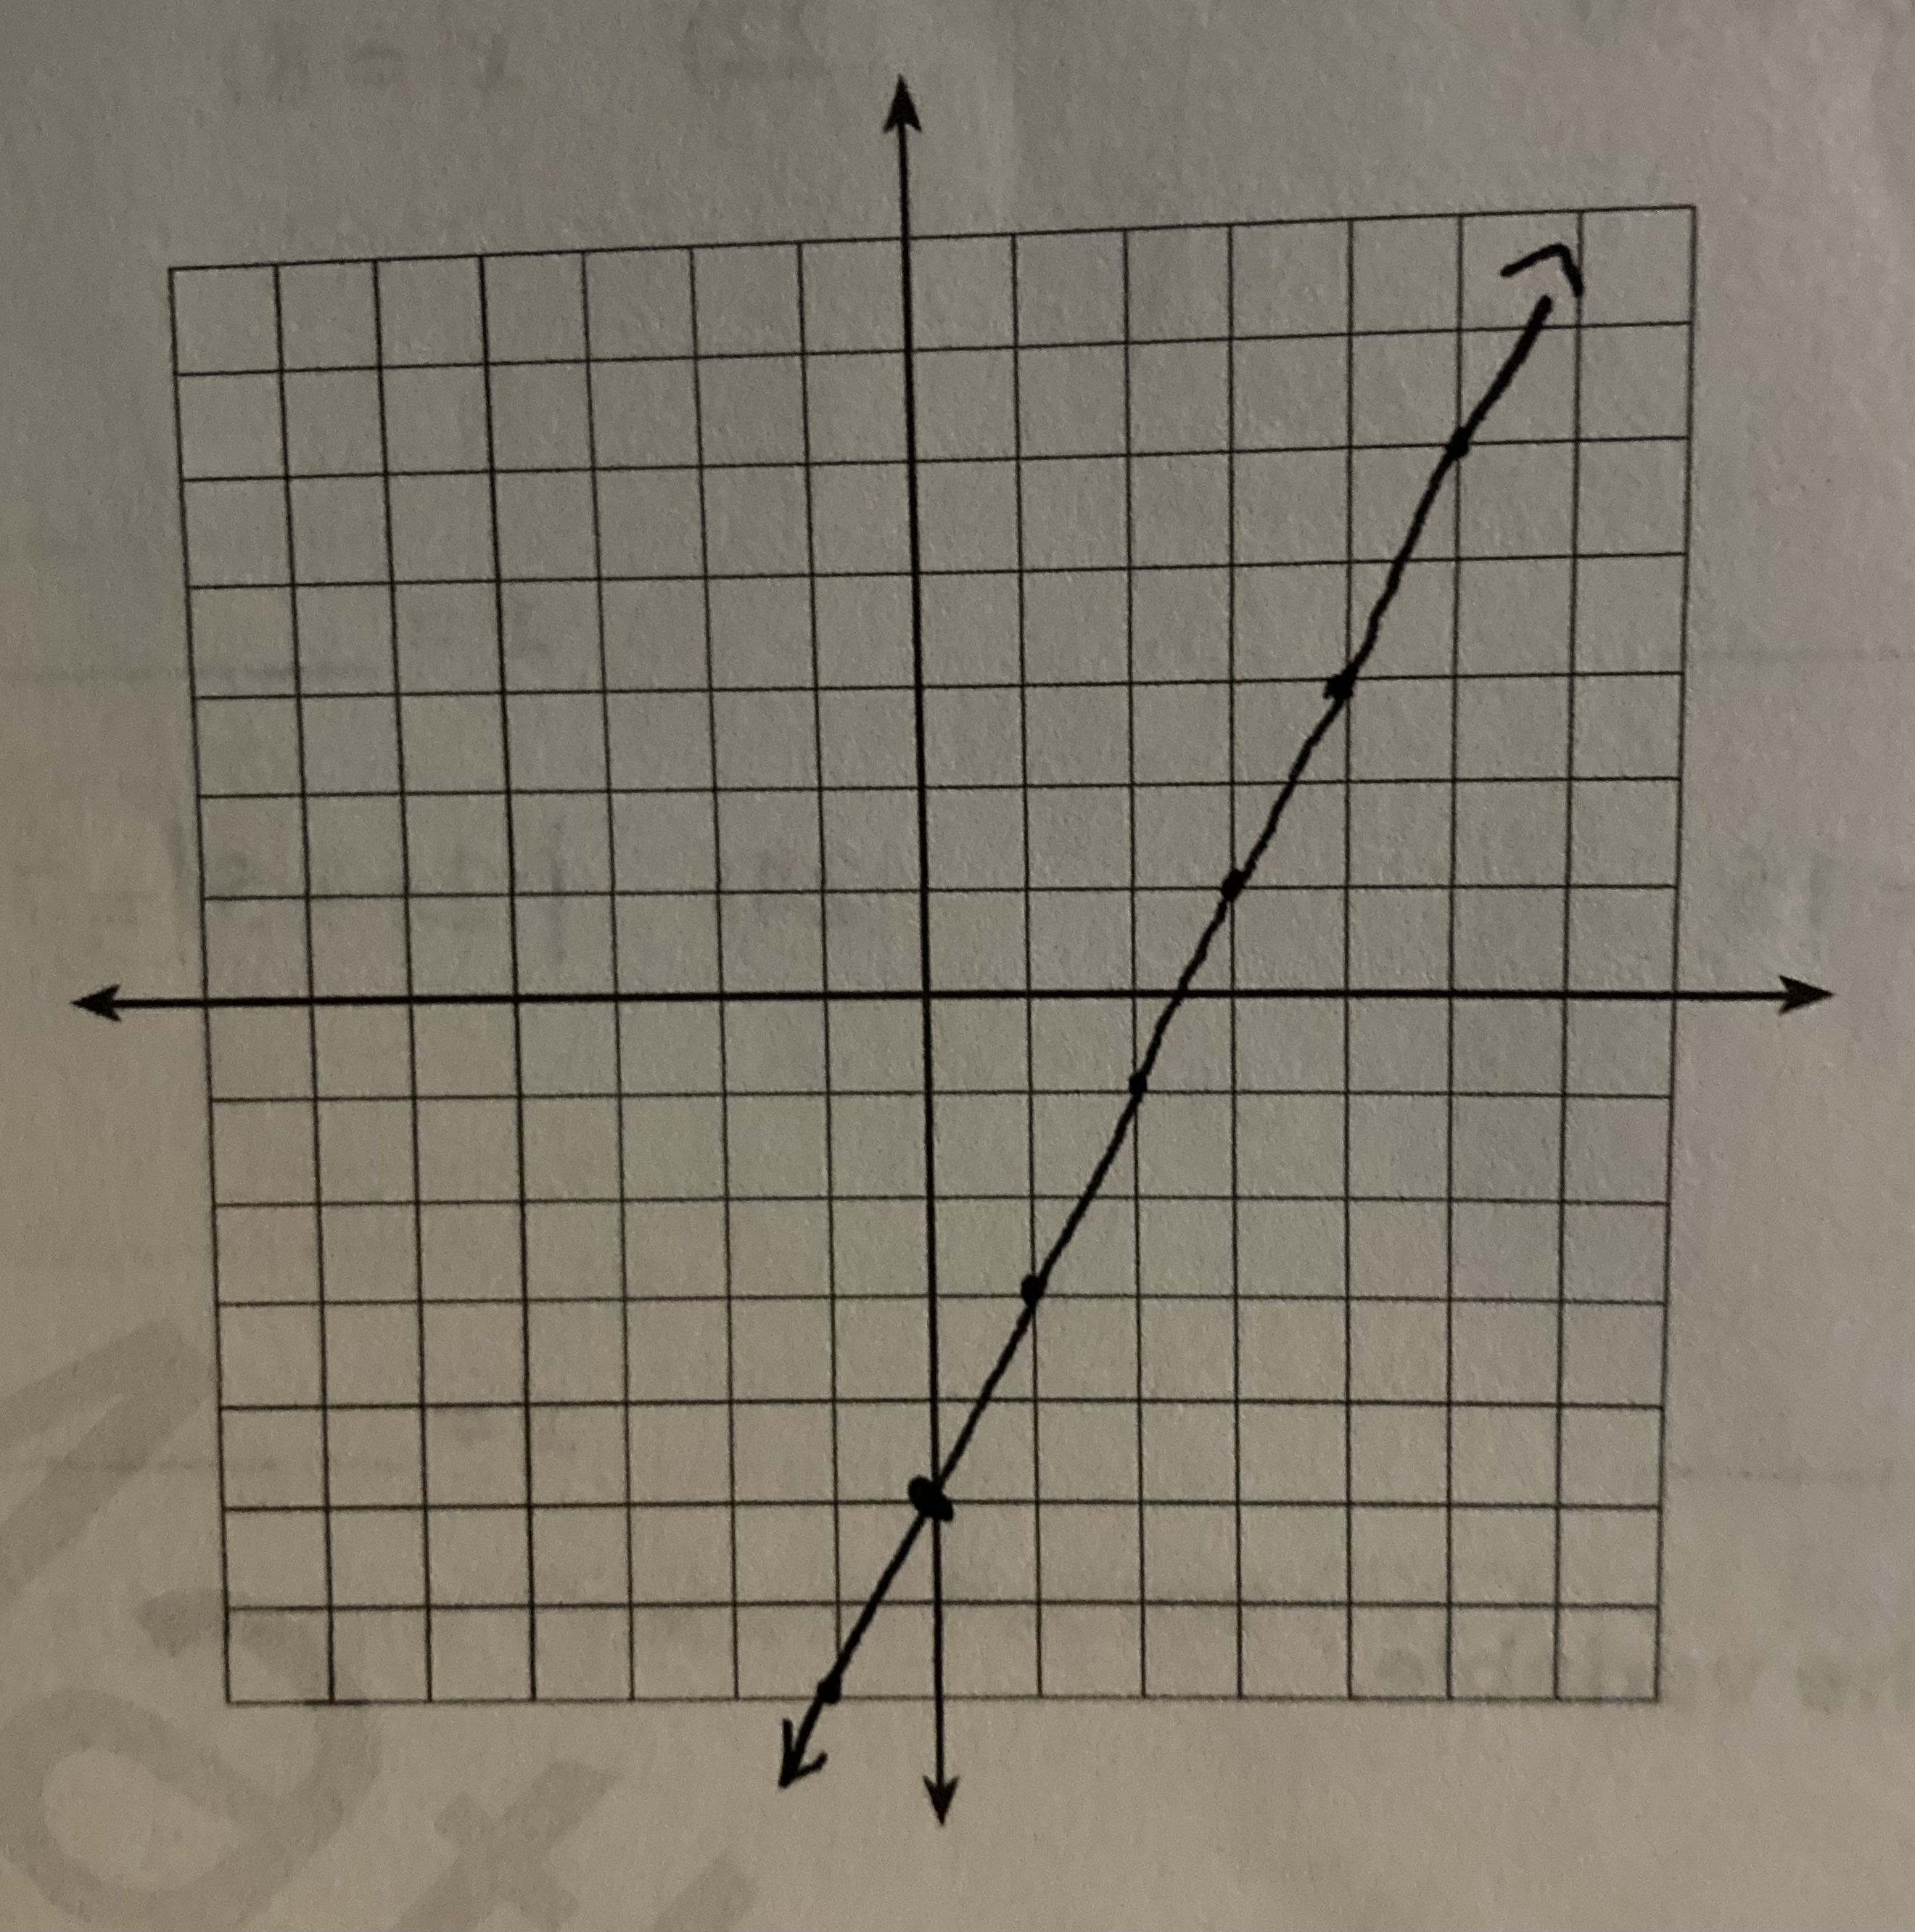
\includegraphics[width = 0.5 \textwidth]{29}
    \end{center}
    \end{proof}
\item  Graph the equation \( 6x + 2y = 12\).
    \begin{proof}[Solution]
    The equation can be re-written in standard form as 
    \[ y = \frac{1}{2}(12 - 6x) = 6 - 3x\]
    which is graphed as follows
    \end{proof}
    \begin{center}
        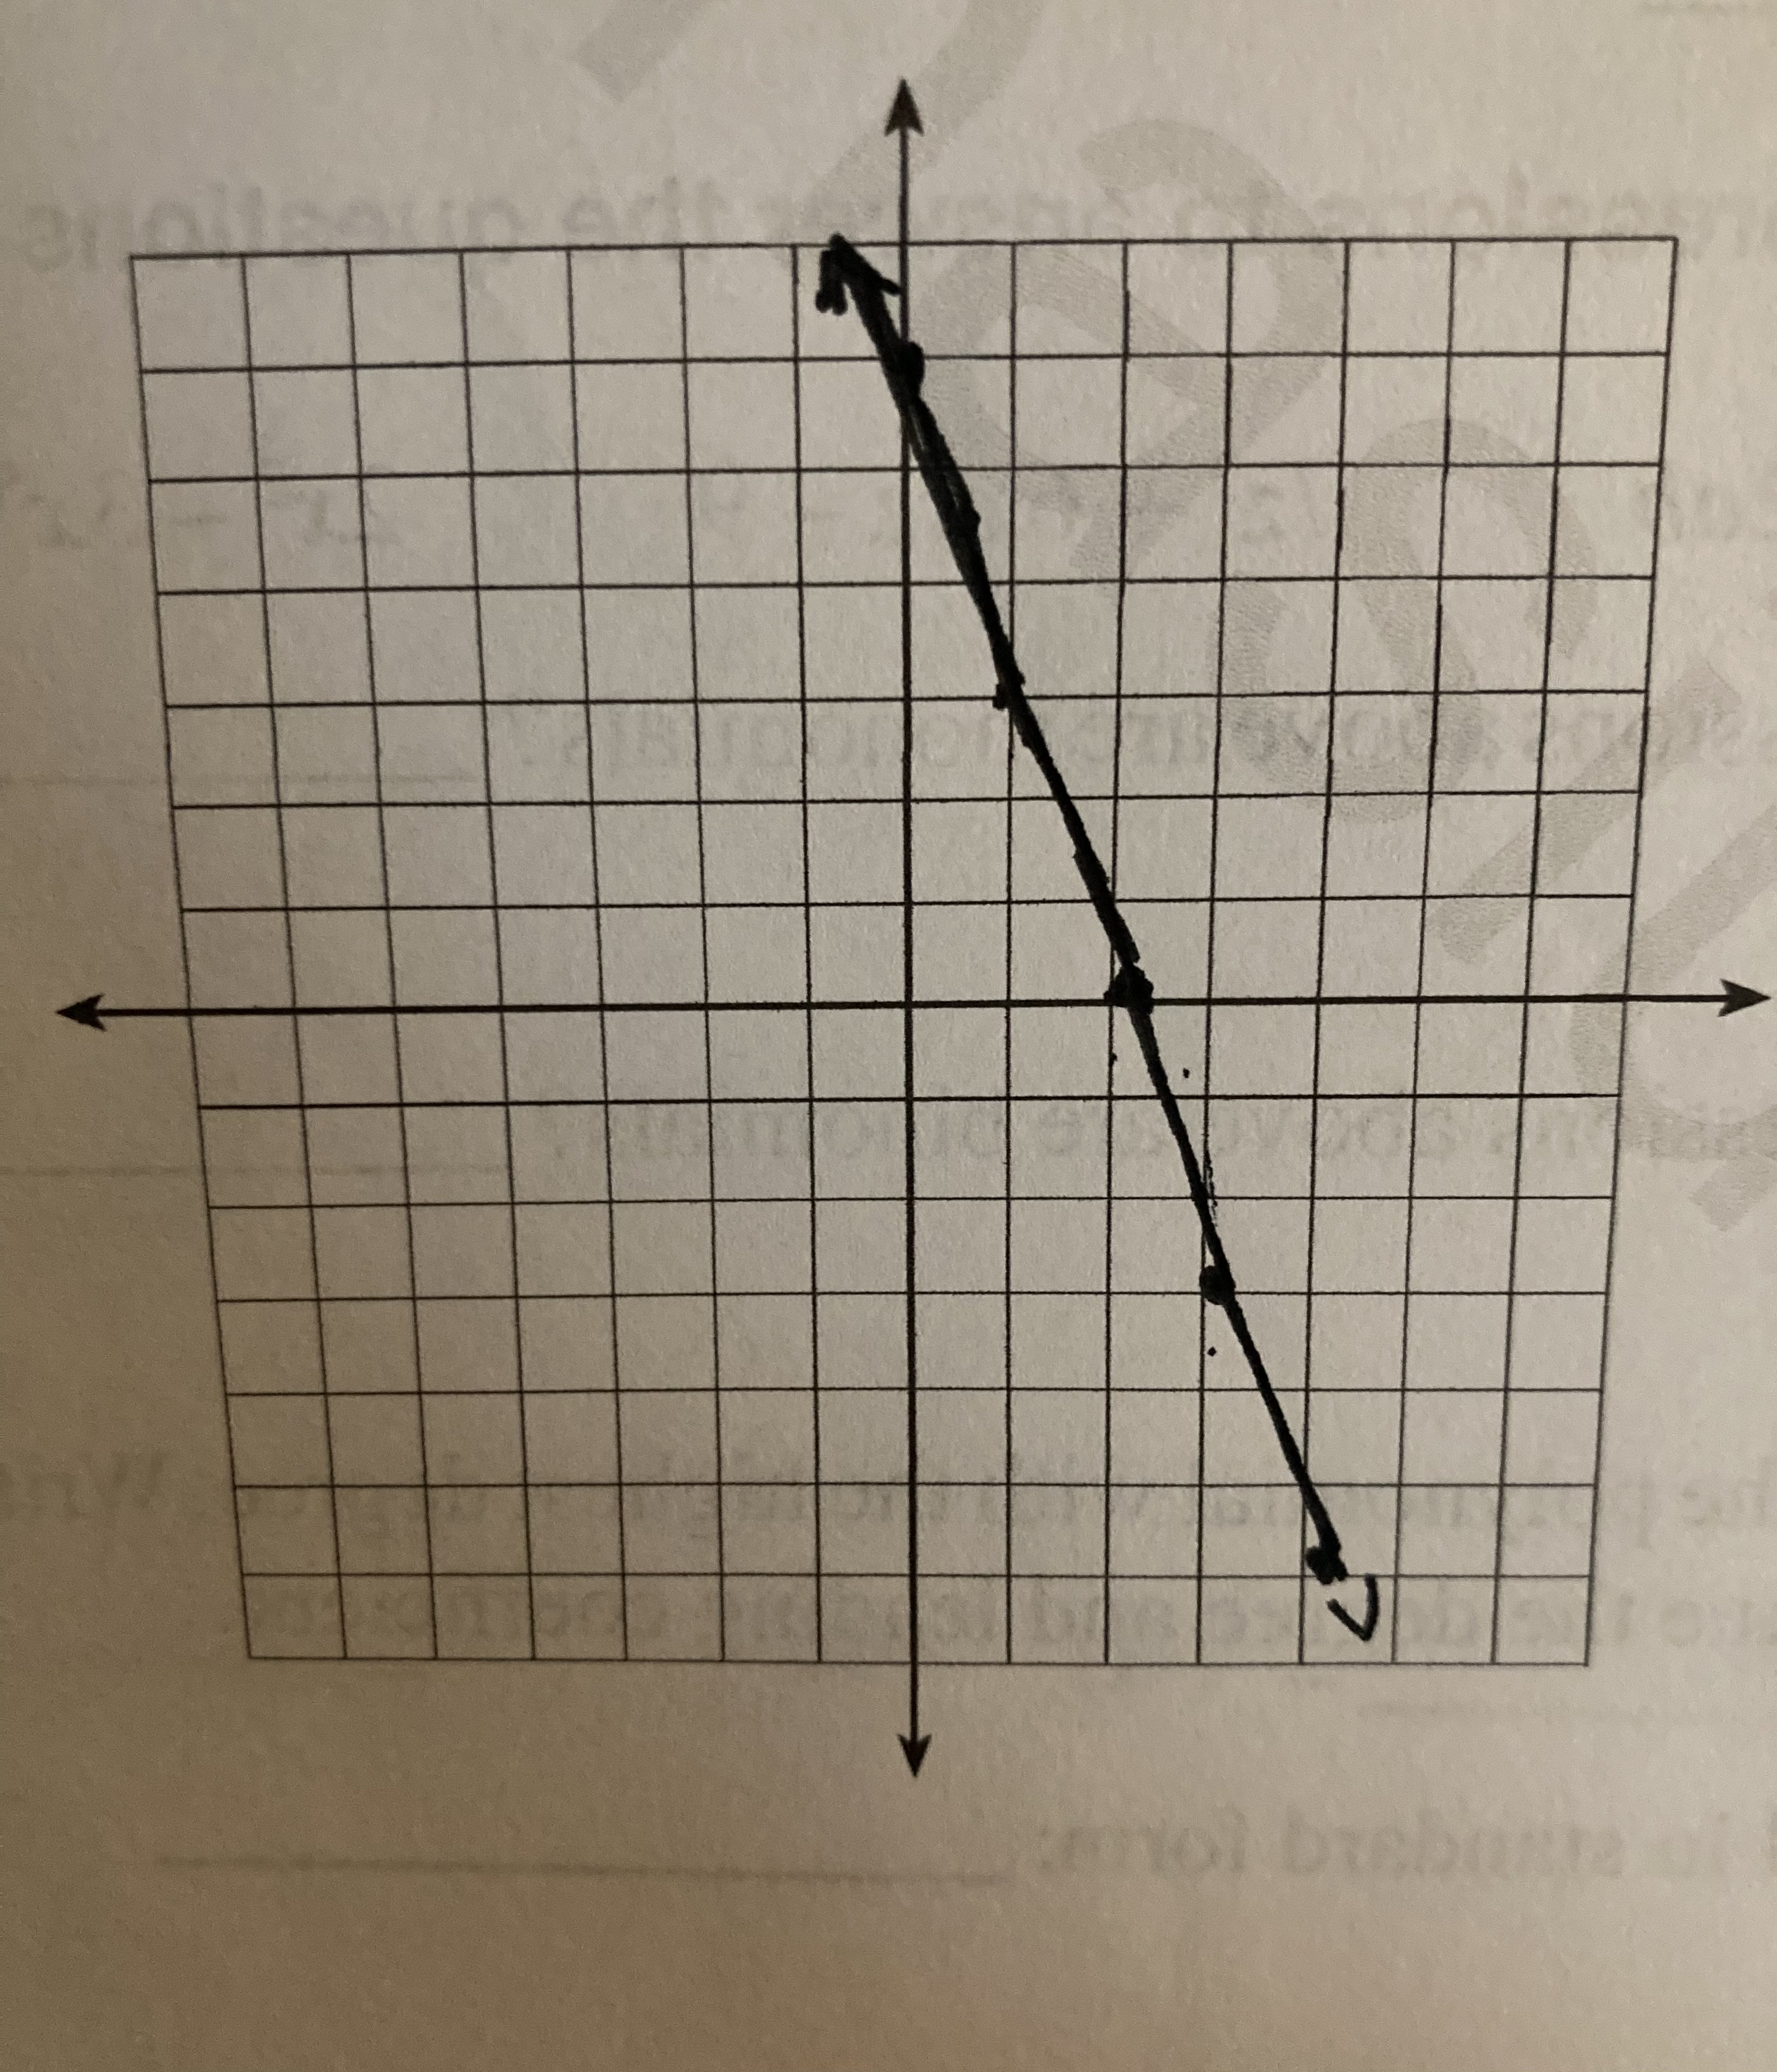
\includegraphics[width=0.5 \textwidth]{30}
    \end{center}
\item Graph the equation \( y - 5 = -\frac{5}{2}(x+1)\).
    \begin{proof}[Solution]
    The equation in slope-intercept form is \( y = \frac{-5}{2}x + \frac{5}{2}.\) and the graph is 
    \end{proof}
    \begin{center}
        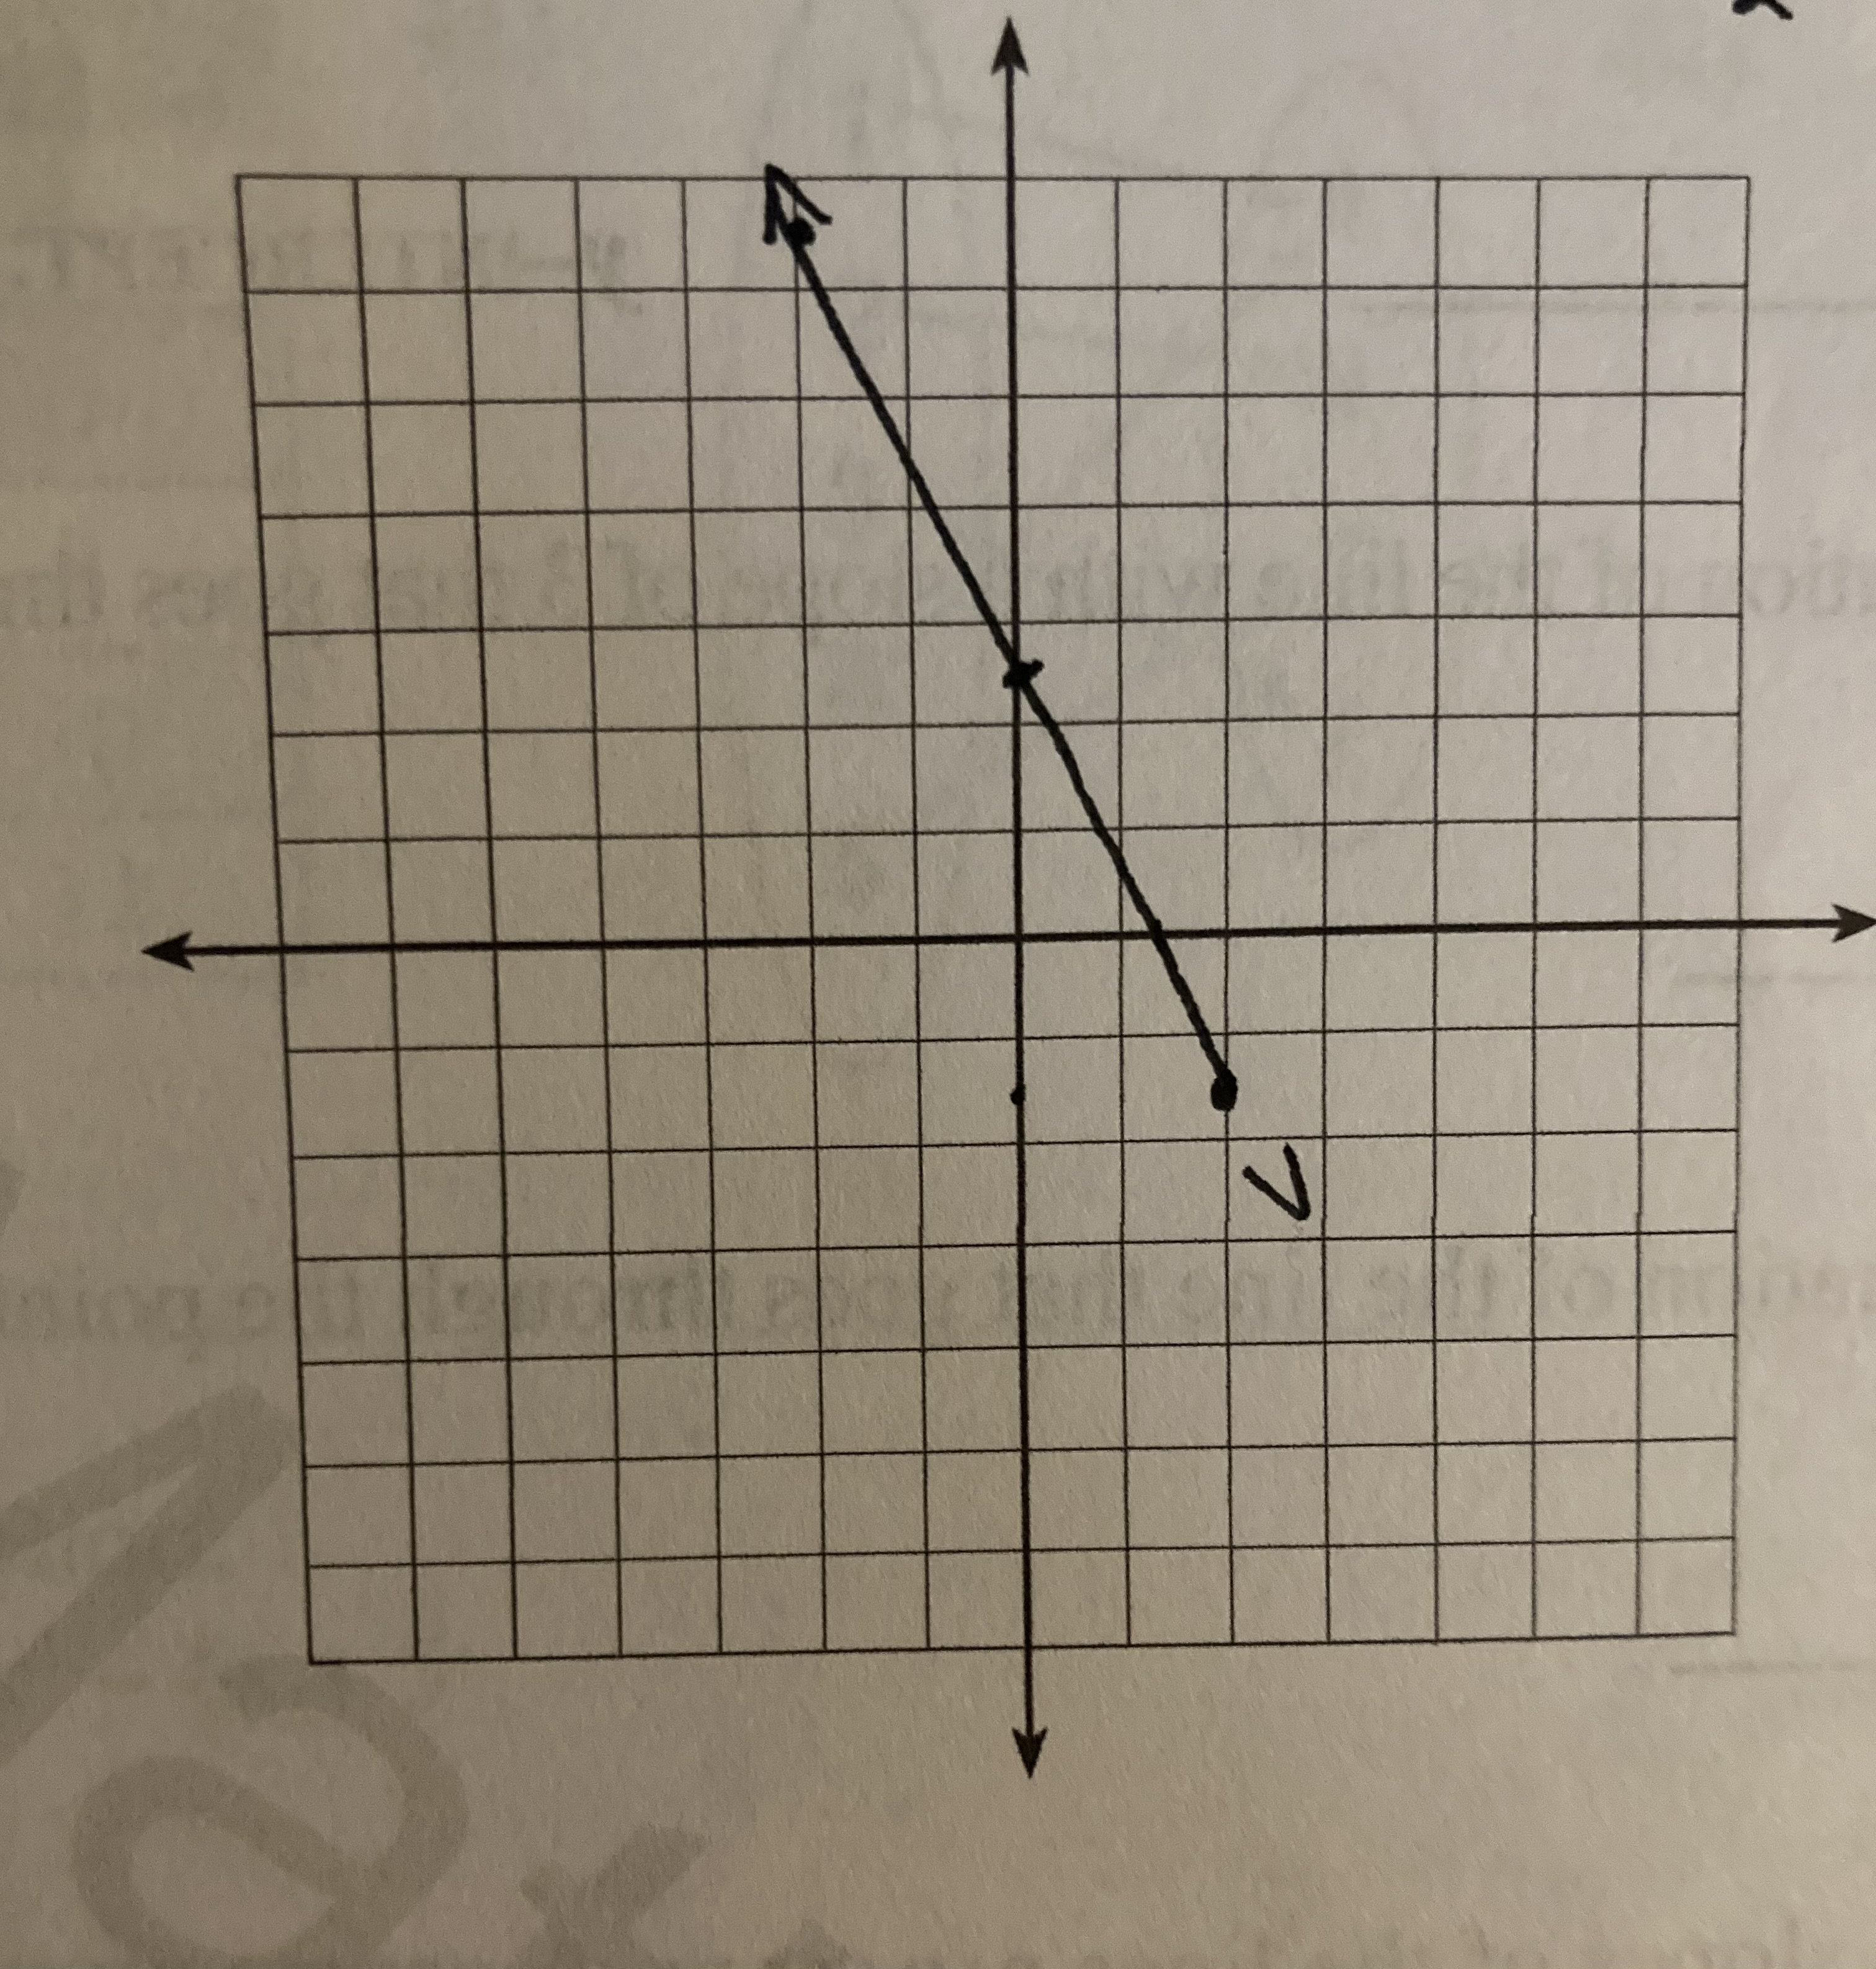
\includegraphics[width = 0.5 \textwidth]{31}
    \end{center}
\item What is the equation of the given line in slope-intercept form?

    \begin{center}
        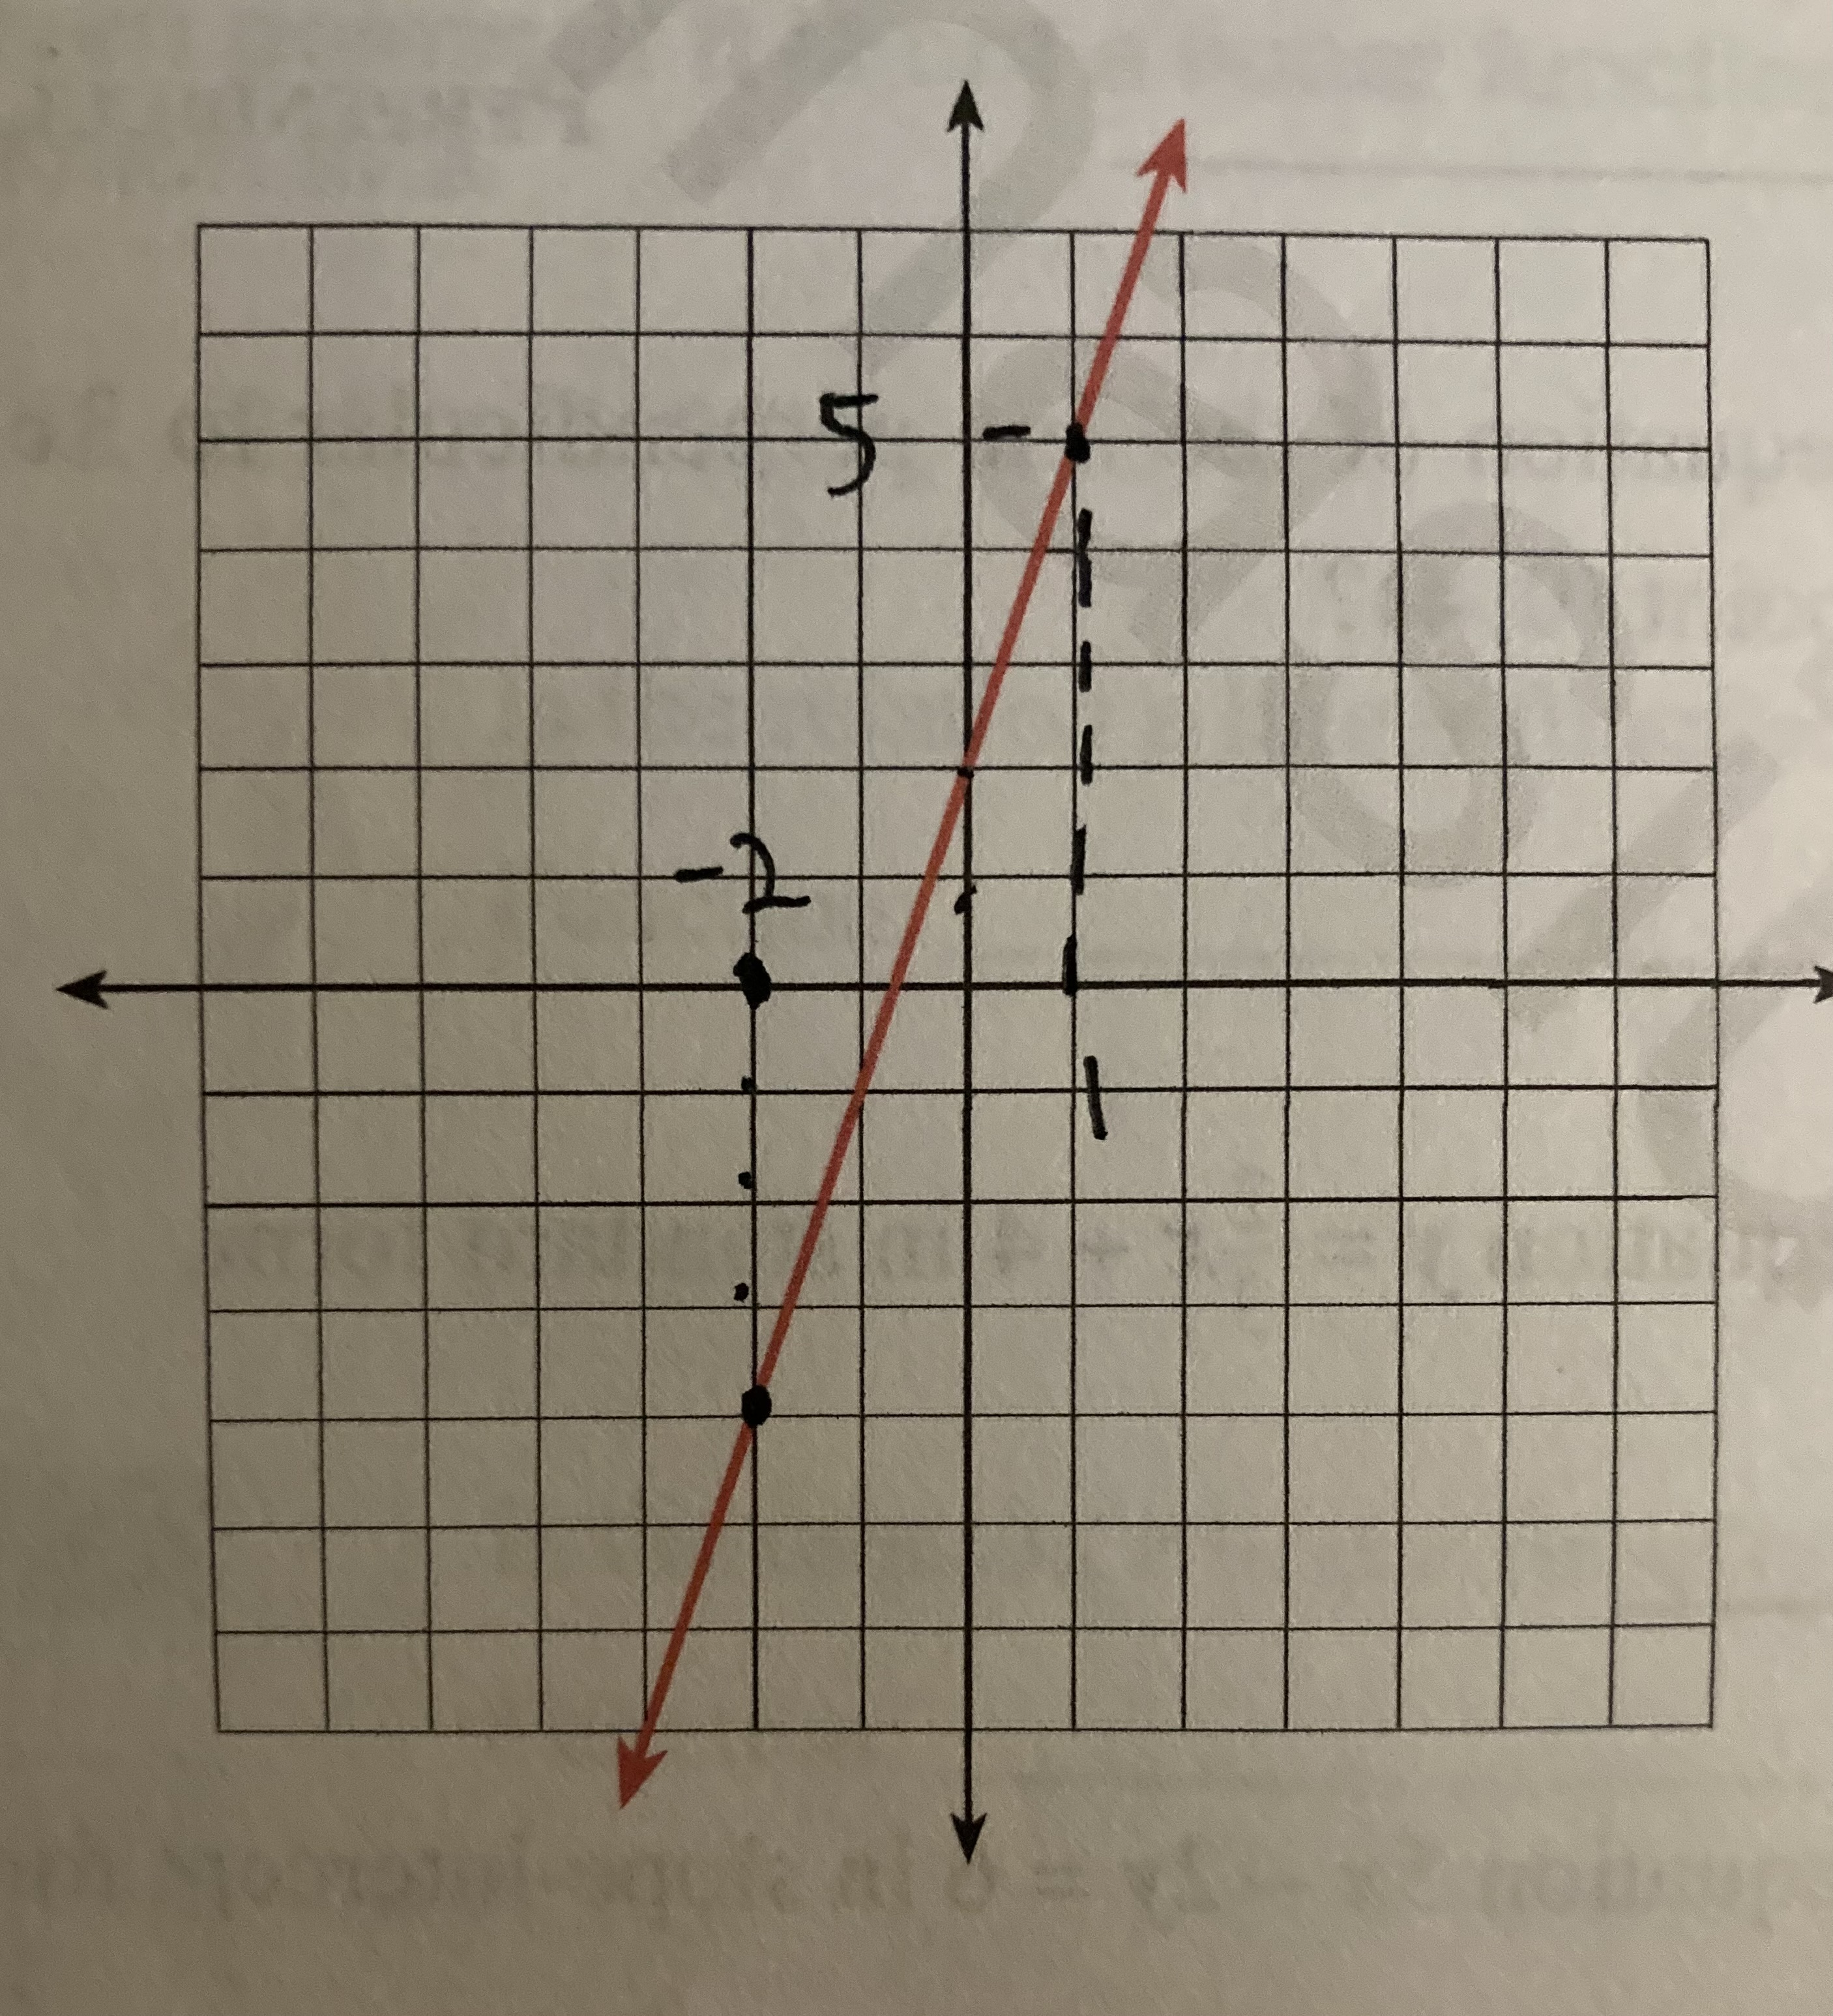
\includegraphics[width = 0.5 \textwidth]{32}
    \end{center}
    
    \begin{proof}[Solution]
    Suppose we start with the slope-intercept form for a line \( y = mx + b \). Pick the point \( (1,5)\) from the graph. Since the \(y-\) intercept is \( b = 2\). We can solve for \( m \) to get the slope of the line. Hence,
    \[ 5 = m + 2 \iff m = 3 \]
    so the equation of the line is 
    \[ y = 3x + 2.\]
    \end{proof}
\item Determine the slope and the coordinate of the \(y-\)intercept of the line given by the equation \( y = 4x - 7 \).
    \begin{proof}[Solution]
    The \textit{slope} of \( y = 4x - 7 \) is \( m = 4 \) and the \textit{coordinate} of the \(y-\)intercept is \( (0,-7)\).
    \end{proof}
\item Write the equation of the line with a slope of \(3\) that goes through the point \( (2,1)\).
    \begin{proof}[Solution]
    Using the slope-intercept form \( y = mx + b \) where \( m = 3 \) is the slope, we can write
    \[ y = 3x + b. \tag{1}\]
    We can solve for \( b \) to get the \(y-\)intercept by substituting the coordinate pair \( (2,1)\) into (1) by writing
    \[ 1 = 3(2) + b \iff b = 1 - 6 = -5 \]
    Hence, we have the linear equation 
    \[ y = 3x - 5.\]
    \end{proof}
\item Write the equation of the line that goes through the points \( (1,2)\) and \((3,-5)\). 
    \begin{proof}[Solution]
    We can take the average rate of change \( y_2 - y_1 = m(x_2 - x_1)\) to find the slope \( m \) of the linear equation 
    \[ y = mx + b. \tag{1}\]
    Plugging the points \((x_1,y_1) = (1,2)\) and \( (x_2, y_2) = (3,-5)\) and solving for \( m \), we get 
    \[ m = \frac{y_2-y_1}{x_2 - x_1} = \frac{-5 - 2 }{ 3 - 1 } = \frac{-7}{2}.\]
    We can take the \(y-\)intercept of (1) by plugging in either of the points above. We choose \((1,2)\) and solving for \(b\) in (1), we have
    \[ 2 = \frac{-7}{2}x + b \iff b = 2 + \frac{7}{2} = \frac{11}{2}.\]
    Therefore, we have 
    \[ y = \frac{-7}{2}x + \frac{11}{2}.\]
    \end{proof}
\item What are the slopes of the lines \textit{parallel} and \textit{perpendicular} to 
    \[ y = 2x - 3. \tag{1}\]
    \begin{proof}[Solution]
    The slope of lines that are parallel to (1) is \( m = 2 \) and slope of lines that are \textit{perpendicular} to (1) is \( m = -1/2\).
    \end{proof}
\item What is the equation of the line perpendicular to \[ 3x + 5y = 15 \tag{1}\] that goes through the point \((0,4)\)?
        
    \begin{proof}[Solution]
    First we put (1) in slope-intercept form by solving for \(y\). Observe that 
    \begin{align*}
        3x + 5y &= 15  \\
        \implies y &= \frac{1}{5}(15 - 3x) \\ 
        \implies y &= 3 - \frac{3}{5} x. 
    \end{align*}
    Since the slope of (1) is \( m = -3/5 \), we must have that the slope of a line perpendicular to it is \( m' = 5 / 3\). Since this perpendicular line goes through \( (0,4 )\), we just have
    \[ y = \frac{5}{3}x + 4.\]
    \end{proof}
\item Rewrite the equation \[ y = \frac{2}{3}x + 4 \tag{1} \] in standard form.
    \begin{proof}[Solution]
    Our goal is to write (1) into the following form 
    \[ ax + by = d.\]
    Hence, (1) becomes 
    \begin{align*}
        3y &= 2x + 12 \iff 3y - 2x = 12. \\
    \end{align*}
    Therefore, the standard form of (1) is 
    \[ -2x + 3y = 12.\]
    \end{proof}
\item Rewrite the equation 
    \[ 5x - 2y = 6 \tag{1}\] in slope-intercept form.
    \begin{proof}[Solution]
    To put (1) into slope-intercept form, we solve (1) for \(y\) in terms of \(x\). Hence, we have \[ 5x -2y = 6 \iff y = -\frac{1}{2} (6 - 5x) = \frac{5}{2}x - 3.\]
    Hence, the slope-intercept form of 
    \[ y = \frac{5}{2}x - 3.\]
    \end{proof}
Determine if the relation is a function. 

\item This is \textbf{NOT} a function. 
\item This is a function.
\item This is \textbf{NOT} a function.
\item Evaluate the function
    \[ f(x) = 3x^2 - 4x + 5\]
at \( x = 2 \). 
\begin{proof}[Solution]
\[ f(2) = 3(2)^2 - 4(2) + 5 = 12 - 8 + 5 = 9.  \]
So \( f(2) = 9 \).
\end{proof}

Determine whether the relation is a linear function. If it is, determine the linear function from the given points. If it is not a linear function, write "not a linear function" on the function line.
\item \( \{ (0,3), (1,6), (2,9), (3,12), (4,15) \}\)
\begin{proof}[Solution]
Yes, this is a linear function and the function is defined as follows:
\[ y = 3x + 3 \]
\end{proof}
\item % Insert table here
\begin{proof}[Solution]
    This is \textbf{NOT} a linear function.
\end{proof}

Determine the domain and range for the relations.
\item \( (2,3), (4,5), (6,7), (8,9)\)
    \begin{proof}[Solution]
        The domain is \( \mathcal{D} = \{x \in \R : 2 \leq x \leq 8  \}\) and the range is \( \mathcal{R} = \{ y \in \R : 3 \leq y \leq 9  \}\). 
    \end{proof}
\item 
    \begin{proof}[Solution]
        The domain is \( \mathcal{D} = (-\infty, 0 ]\) and the range is \( \mathcal{R} = (-\infty, +\infty)\).
    \end{proof}
\item The amount of water left in a \( 30 \) liter tank can be modeled by the equation 
    \[ w = -\frac{1}{2}t + 30, \]
    where \( w \) is the \textit{amount of water left in the tank} and \( t \) is \textit{time in hours} since the water in started leaking. Water leaks from the tank until the tank is empty. Determine the domain and range of this scenario.
    \begin{proof}[Solution]
        The domain in this scenario is \( \mathcal{D} = \{ t \in \R: 0 \leq t \leq 60  \}\) where \(t\) is in hours and the range is \( \mathcal{R} = \{ w \in \R : 0 \leq w \leq 30 \}\) where \(w\) is in liters.
    \end{proof}

    Graph the solutions.
\item \( -1 < 2x + 5 < 9 \) 
    \begin{proof}[Solution]
    First we solve for \(x\). So 
    \begin{align*}
        -1 < 2x+5 < 9  \\
        \implies -6 < 2x < 4 \\
        \implies -3 < x < 2
    \end{align*}
    So graphing this on would look like 
    %insert figure here
    \end{proof}
    \begin{center}
        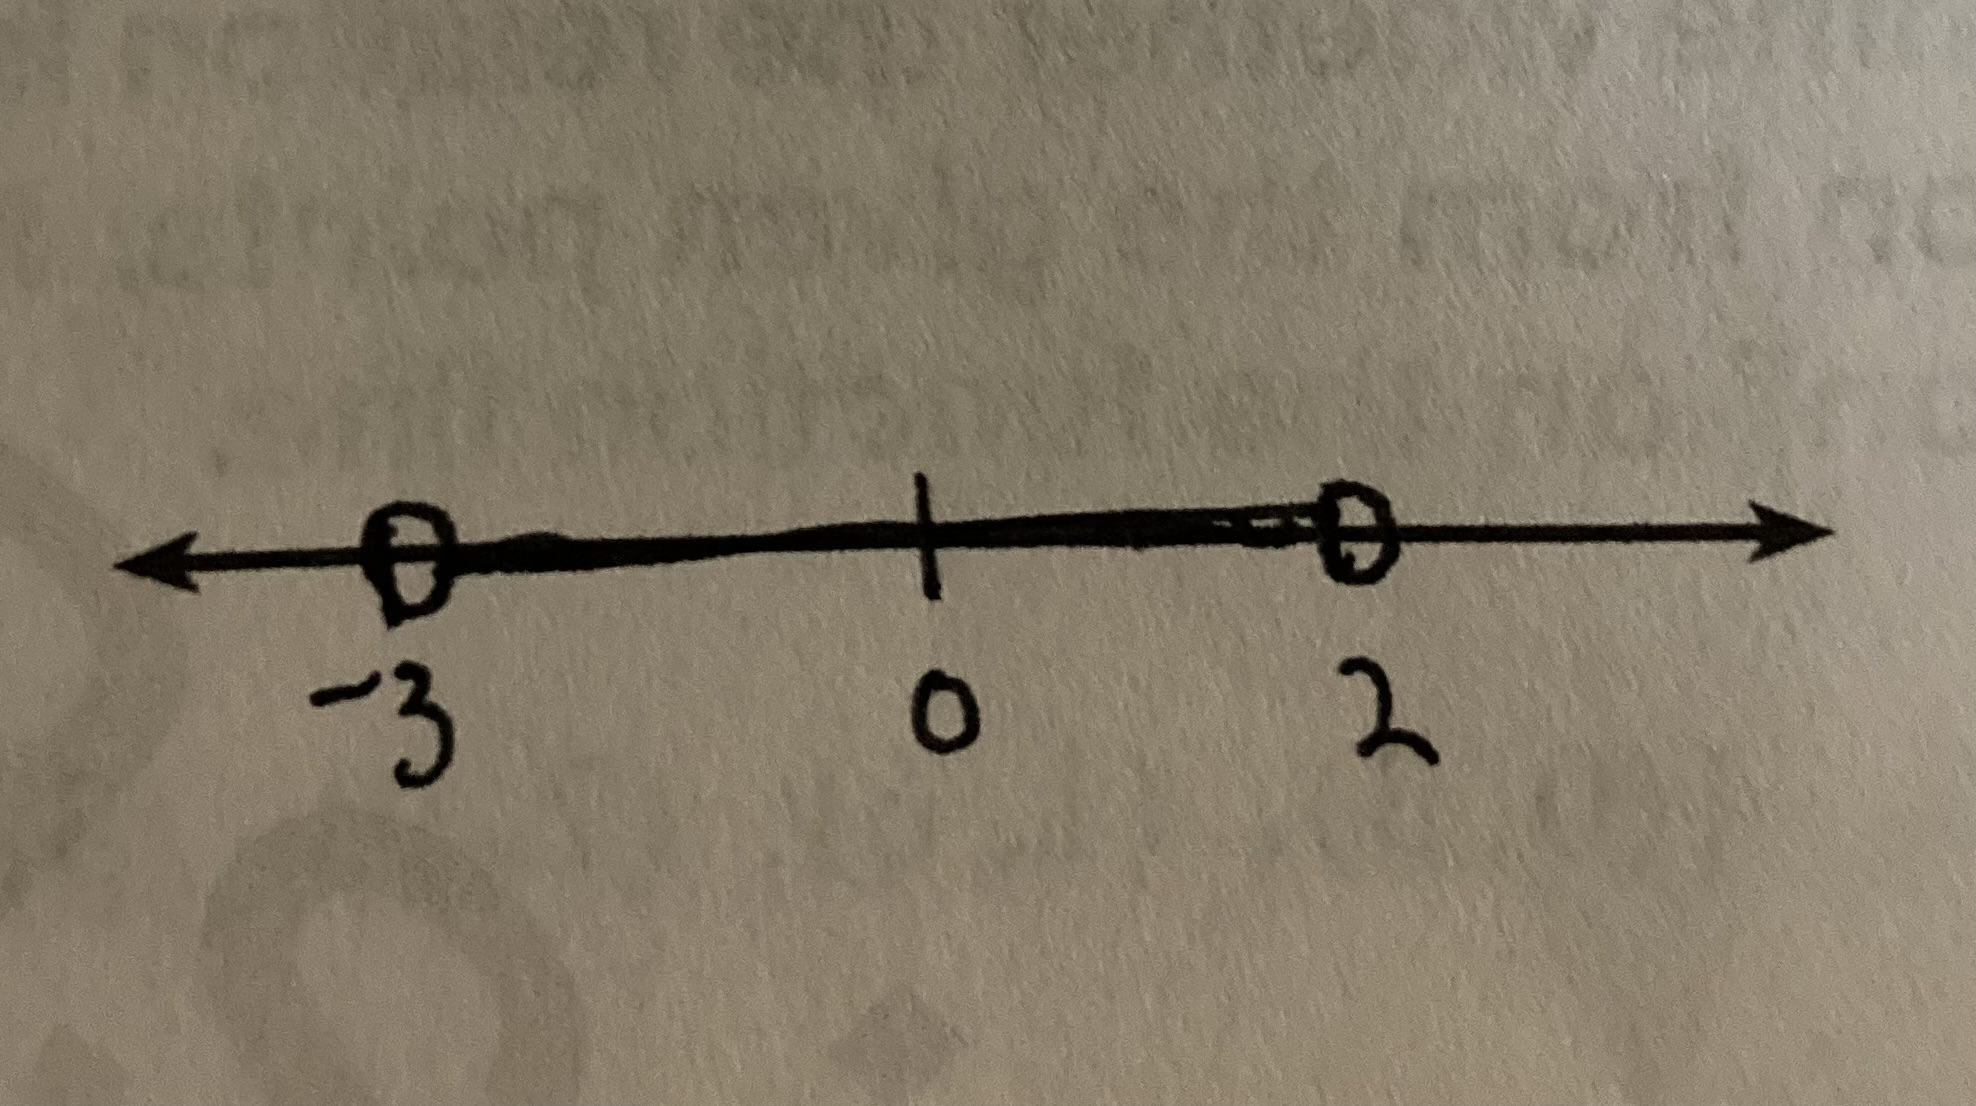
\includegraphics[width = 0.5 \textwidth]{49}
    \end{center}
\item \( 4x+7 \leq -13 \) or \( 5x+4 \geq 14\).
    \begin{proof}[Solution]
    Again, we solve for \( x \) for \( 4x + 7 \leq -13  \) and \( 5x + 4 \geq 14\). Starting with the former, we have 
    \[ 4x + 7 \leq -13 \iff x \leq \frac{-20 }{4} = -5. \]
    For the latter, we have 
    \[ 5x + 4 \geq 14 \iff x \geq \frac{10}{5} = 2.\]
    Hence, we have \( x \leq -5 \) or \( x \geq 2 \). Graphing this looks like
    \begin{center}
        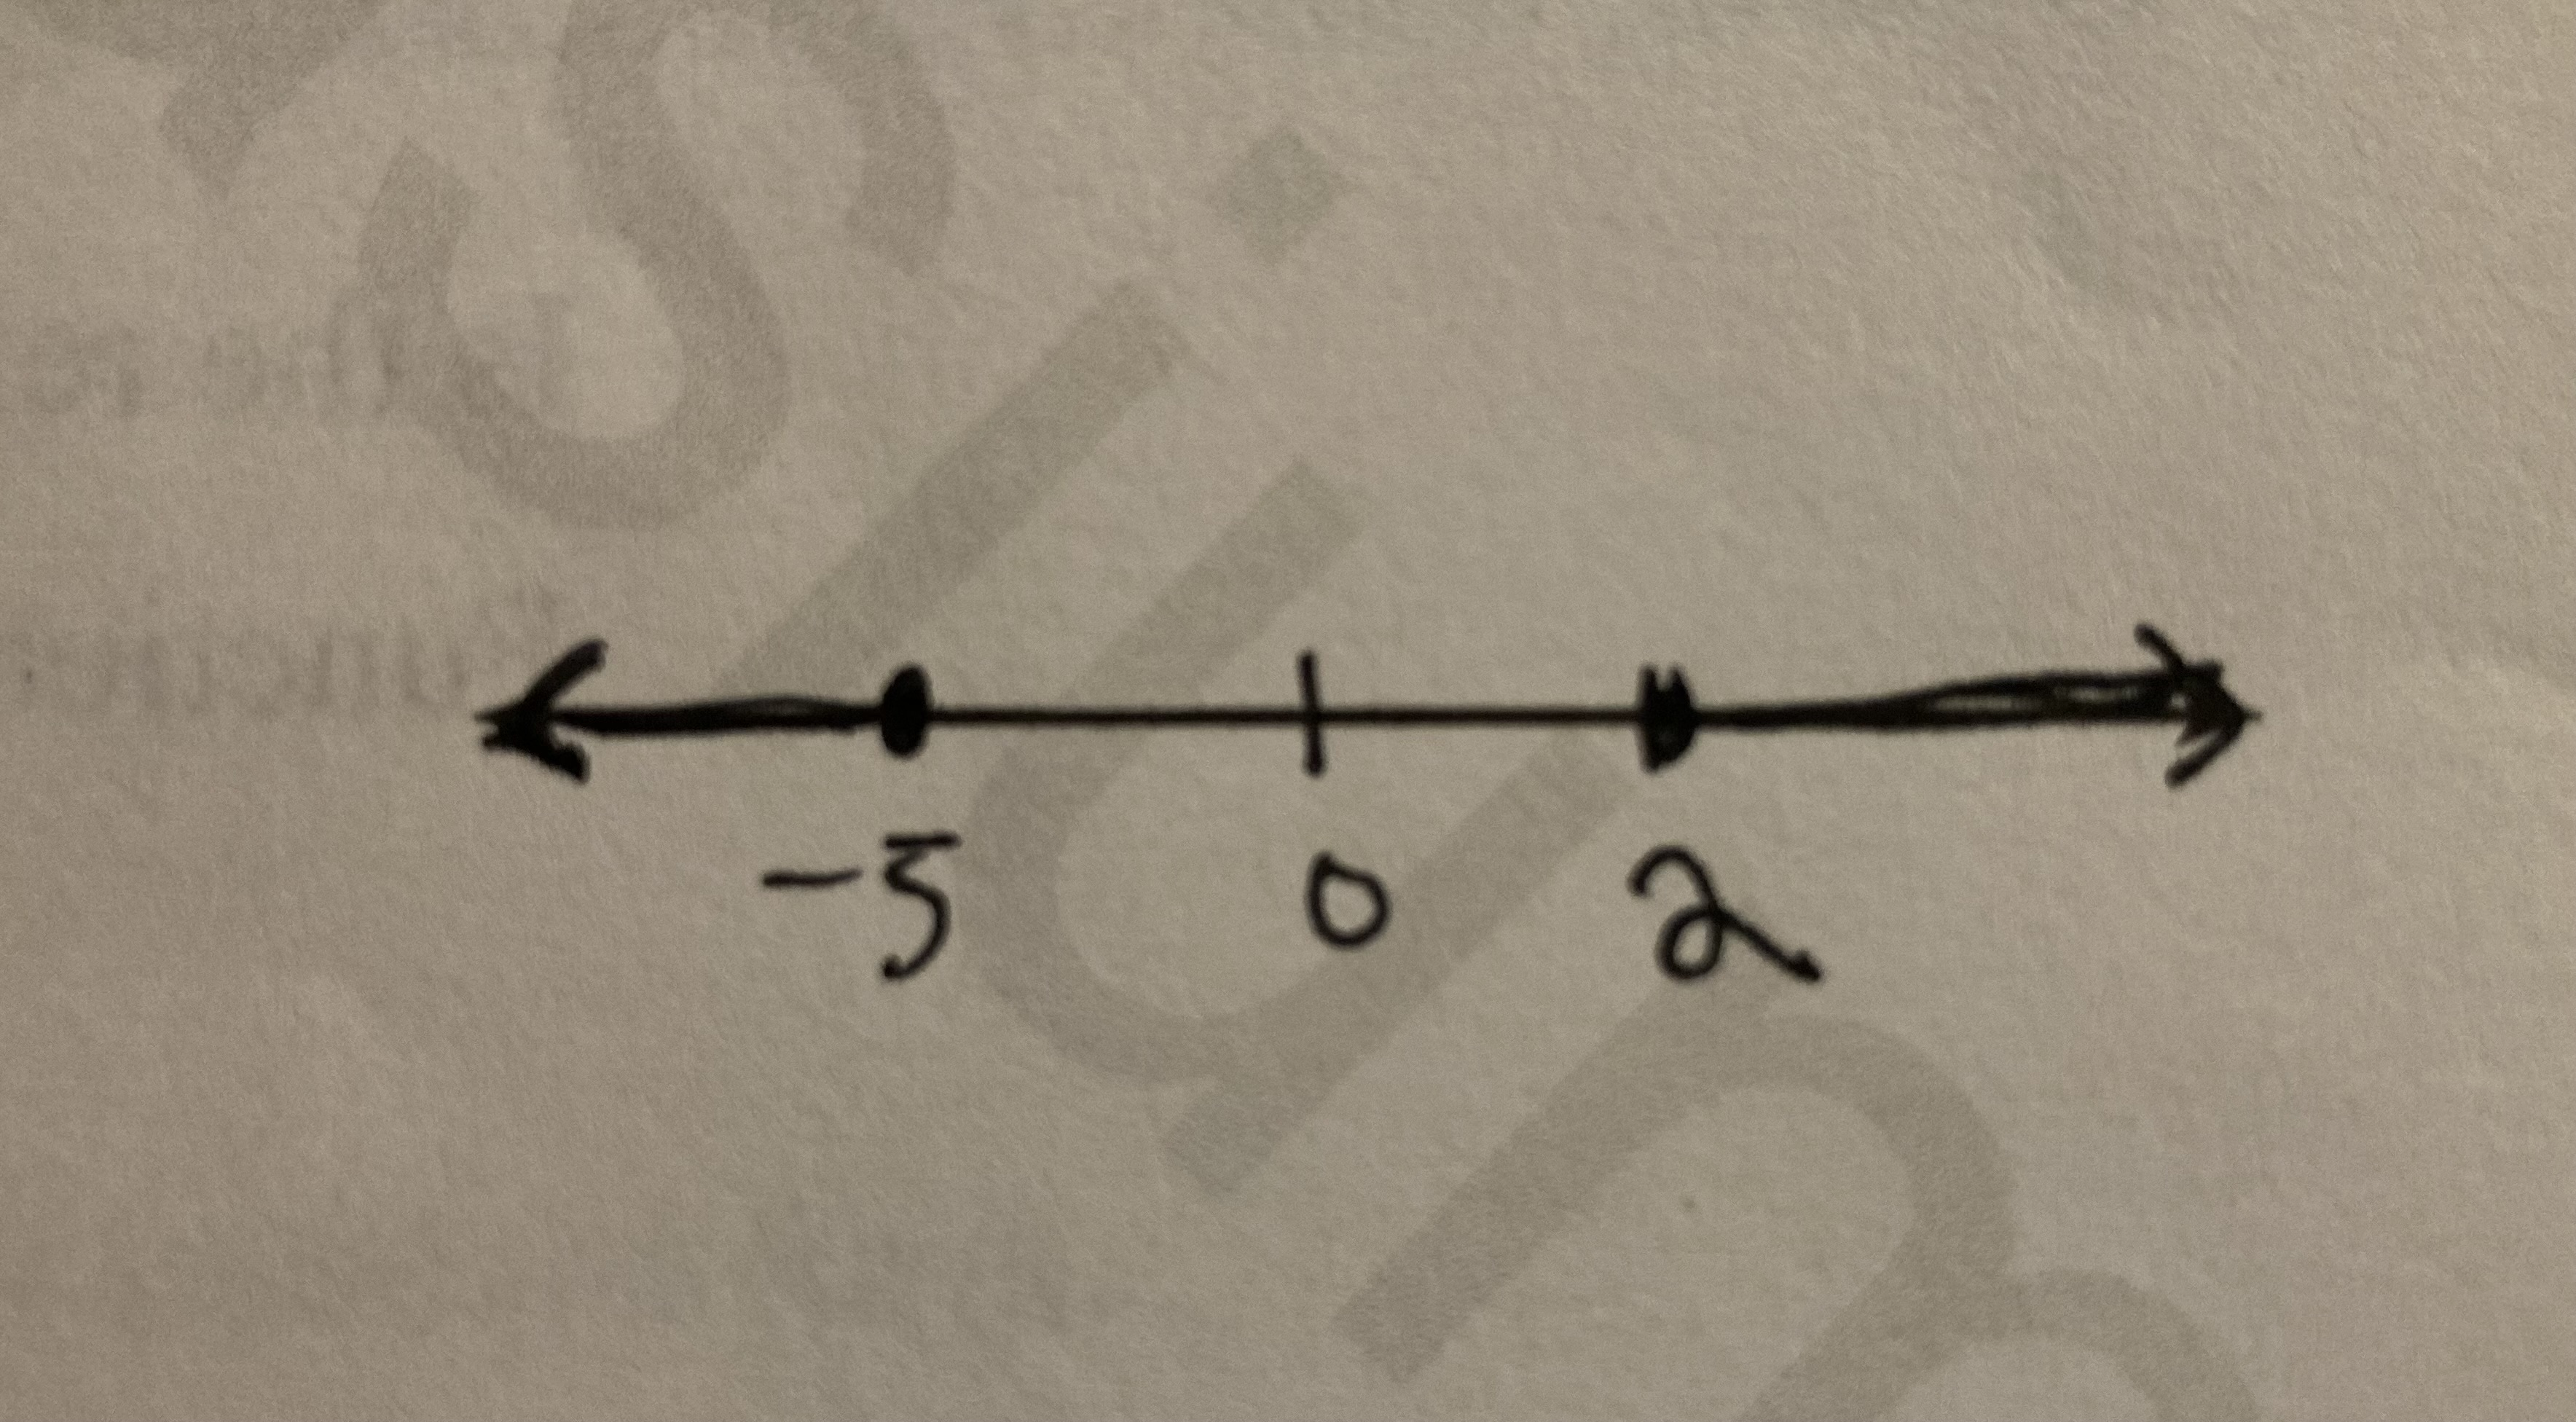
\includegraphics[width = 0.5 \textwidth]{50}
    \end{center}
    \end{proof}
\item \( |8x-4| \leq 28\)
    \begin{proof}[Solution]
    By definition of absolute value, we have 
    \begin{align*}
        |8x - 4 |\leq 28 \\
     -28 \leq 8x - 4 \leq 28 \\
      -24 \leq  8x \leq 32  \\
      \iff -3 \leq x \leq 4 \tag{1}.
    \end{align*}
    Hence, graphing (1) leads to 
    %insert graph
    \begin{center}
        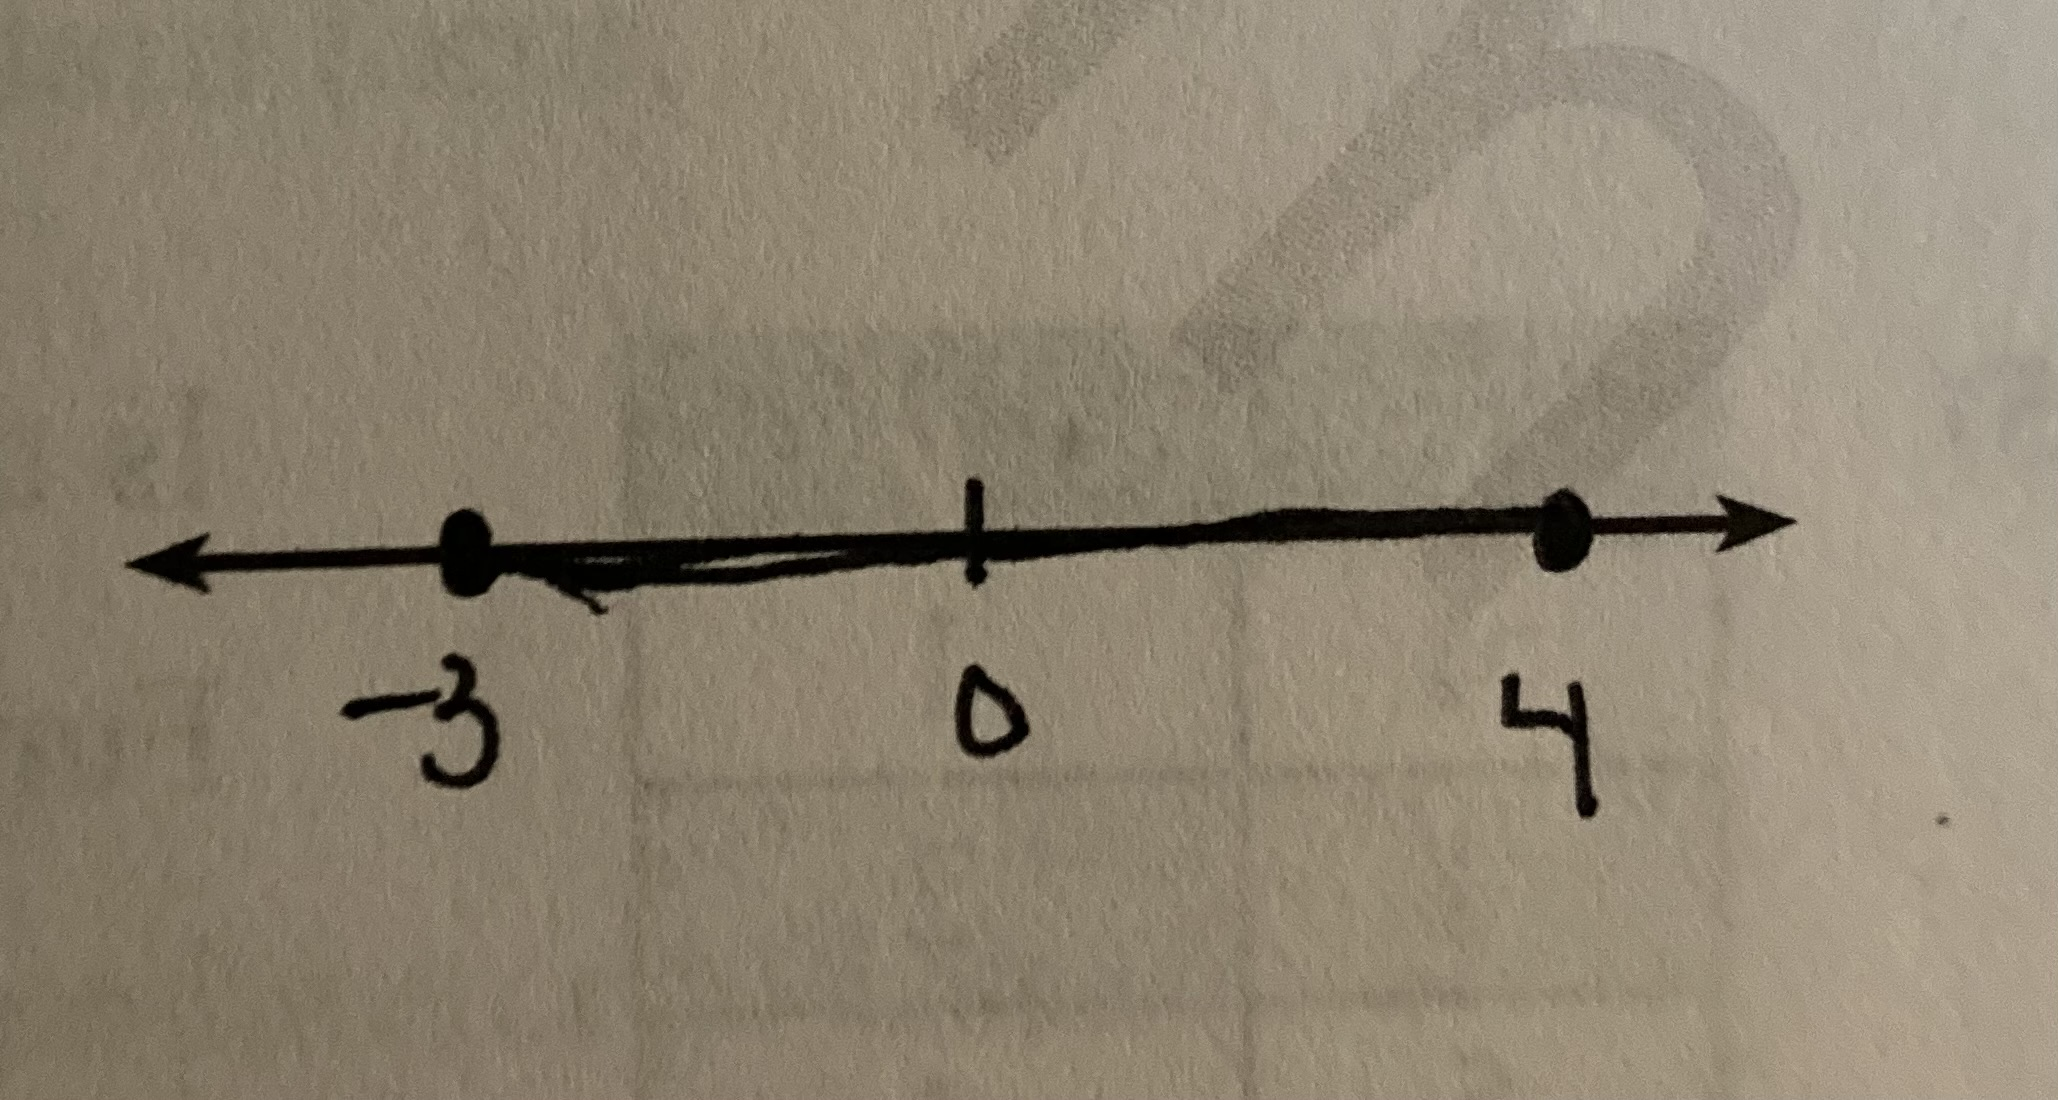
\includegraphics[width = 0.5 \textwidth]{51}
    \end{center}
    \end{proof}
\item The sum of three consecutive odd integers is 195. What are the three integers?  
    \begin{proof}[Solution]
    Let \( x \in \R \), then the sum of three consecutive odd numbers can be written as 
    \[ x_1 + x_2 + x_3 = (2k + 1) + (2k+3) + (2k + 5 ) = 195. \tag{1} \]
    This implies that 
    \[ 6k + 9 = 195 \iff k = \frac{195-9}{6} = 31. \]
Plugging this back into (1), yields the following consecutive odd integers 
\[ 63, 65, 67.\]
    \end{proof}
\item Deandra has \( \$15 \) more than Elias. Frank has \( 3 \) times as much as Deandra. Together they have \( \$185\). How much does each person have? 
    \begin{proof}[Solution]
    Let \( D, x, F\) be variables that stand for Deandra, Elias, and Frank respectively. By the problem statement, we have the following equations
    \begin{align*}
        D &= x + 15,  \\
        F &= 3D = 3(x+15).
    \end{align*}
    Their total sum is \(  D + F = 4(x+15) = \$ 185\). Since the amount Elias has is unknown, let's solve for \(x    \). Hence, we have 
    \[ 4(x+15) = 185 \iff x = \frac{185}{4} - 15 = \$ 31.25.\]
    So Elias has \( \$ 31.25\), Deandra has 
    \[ D = 31.25 + 15 = \$ 46.25 \]
    and Frank has 
    \[ E = 3D = 3(46.25) = \$ 138.75.\]
    \end{proof}
\item If \( y \) varies inversely with \( x \) and \( y = 2 \) when \( x = 5 \), what is the value of \( x \) when \( y = 3 \)?
    \begin{proof}[Solution]
    Since \( y \) varies inversely with \( x \), we have 
    \[ y = \frac{k}{x} \tag{1}.\]
    where \( k \in \R \) is the constant of proportionality. First we need to find \( k \in \R \). Since \( y = 2 \) when \( x = 5 \), solving for \( k \) yields
    \[ k = y \cdot x = 2 \cdot 5 = 10.\]
    If \( y = 3 \), the value of \( x \) is simply 
    \[ x = \frac{10}{3}.\]
    \end{proof}
Karen can complete 12 coloring book pages in 30 minutes.
\item What is the constant of proportionality in the scenario?
    \begin{proof}[Solution]
    If Karen can complete 12 coloring book pages in 30 minutes, then the constant of proportionality is 
    \[ k = \frac{12}{30} = \frac{2 \text{ coloring books}}{5\text{ minutes}}\]
 
    \end{proof}
\item Write a direct variation equation that represents the scenario.
    \begin{proof}[Solution]
    Let \( x,y \in \R \) and \( k \) constant such that \(x \) represents time in minutes and \(y \) represents the amount of completed coloring books. The situation can be modeled by the equation:
    \[ y = \frac{2}{5}x\]
    \end{proof}
\item How long will it take Karen to complete a 96-page coloring book?
    \begin{proof}[Solution]
    If we solve for \( x \) in the above equation with \( y = 96\) coloring books, then the amount of time in minutes is 
    \[ x = \frac{5}{2} \cdot 96 = 240 \text{ min}.\]
    \end{proof}

\item 5 less than a number. 
    \begin{proof}[Solution]
    This can be written as \( 5 < x \) where \( x \in \R \)
    \end{proof}
\item 7 more than the quotient of \( x \) and 3 is 4.
    \begin{proof}[Solution]
    This can written as \( 7 + \frac{x}{3} = 4\) where \( x \in \R \).
    \end{proof}
Write an equation that models the scenario.
\item The price of a pizza costs \( \$ 15\) plus \( \$ 3 \) for each topping.
    \begin{proof}[Solution]
    Let \( x \in \R \) represent the amount of toppings and let \( y \in \R \) represent the price of the pizza in dollars where \( y(0) = \$ 15 \) is the initial value of the pizza. The equation for this scenario is 
    \[ y = 3x + 15. \]
    \end{proof}
Solve for \(F\).
\item \( 2H - 3F = 4J + 8K \).
    \begin{proof}[Solution]
    Solving for \(F \), we have 
    \[ F = \frac{1}{3}(2H - 4J - 8K ).\]
    \end{proof}
\item \( \frac{5}{9}(F - 32) = C \). 
    \begin{proof}[Solution]
        Solving for \( F \), we have
    \begin{align*}
        &\frac{5}{9}(F-32)= C   \\
        &\implies F - 32 = \frac{9}{5}C \\
        &\implies F = \frac{9}{5}C + 32.
    \end{align*}
    \end{proof}
\item Find the solution to the system of equations 
    \begin{align}
        y&= -\frac{2}{3}x - 3  \\
       y &= 2x + 5.
    \end{align}
    by graphing. Use a straightedge. 
    \begin{proof}[Solution]
    The solution is \( (x,y) = (-3,-1)\) from the graph below:
    \begin{center}
        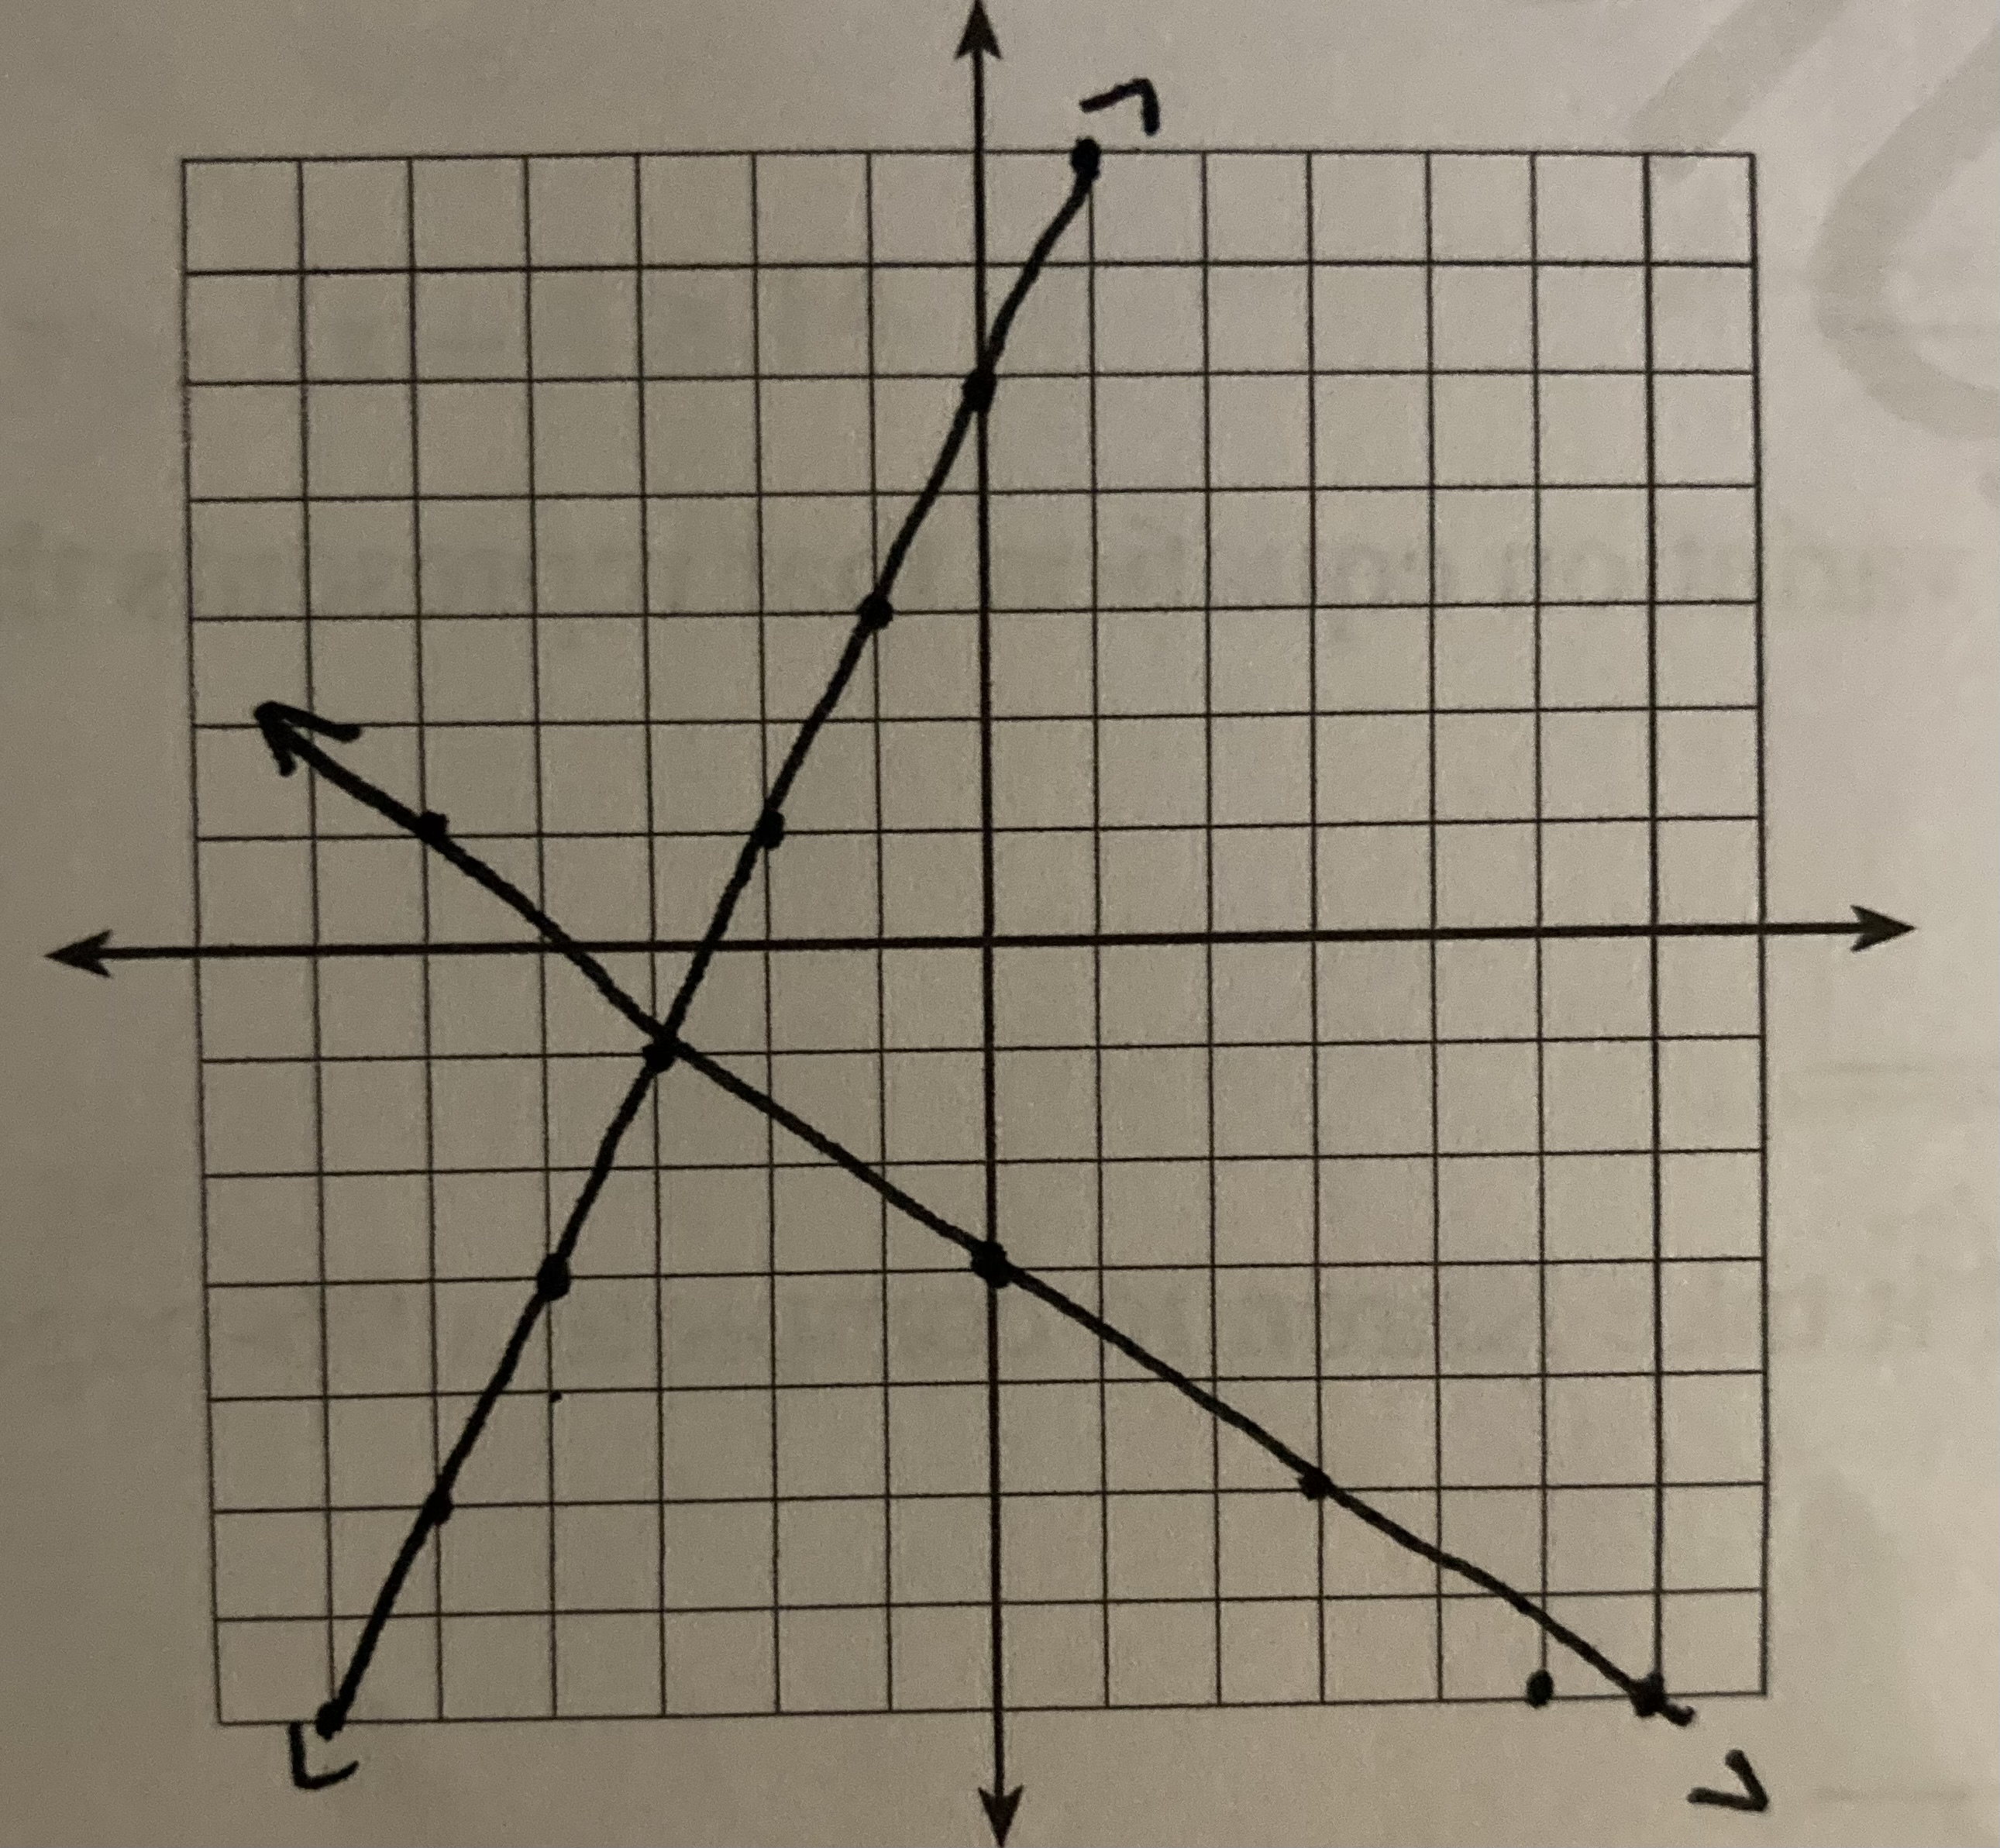
\includegraphics[width = 0.5 \textwidth]{IMG_8426}
    \end{center}
    \end{proof}
Solve the following system of equations.
\item \begin{align*}
    &y = -3x + 13  \\
    &4x + 3y = 29.
\end{align*}
\begin{proof}[Solution]
Rewriting this system yields 
\begin{align*}
    3x + y  &= 13 \tag{1}\\
    4x + 3y &= 29 \tag{2}.
\end{align*}
We can use elimination to to solve for \( x\). Hence, multiply (1) by -3 which yields 
\[ -3(3x + y ) = -3 \cdot 13 \iff -9x -3y = -39. \tag{3}\]
Then we can substract (3) and (2) to get 
\[ -5x = -10 \iff x = 2.\]
To find \(y\), we can plug in \(x\) to either (1) and (2) above. Suppose we solve for \( y \) in (1), then we get 
\[ y = -3(2) + 13 = 7.\]
Hence, the solution for the system of equations above is \( (x,y) = (2,7)\).
\end{proof}
\item \begin{align*}
        2x + 3y &= 8  \tag{1}\\
        5x - 6y &= -7. \tag{2}
\end{align*}
\begin{proof}[Solution]
Multiplying (1) by 2 and adding the result to (2), we get 
\[ 9x = 9 \iff x = 1.\]
We can plug in \( x = 1 \) into (1) and solve for \(y\) by writing
\begin{align*}
    &2x + 3y = 8 \\
    &\implies y = \frac{1}{3} (8 - 2x)\\
    &\implies y = \frac{1}{3} (8 - 2) \\
    &\implies y = 2.
\end{align*}
Hence, the solution to the system of equations above is \( (x,y) = (1,2)\). 
\end{proof}
\item Three T-shirts and four dresses cost \( \$ 125\). Two T-shirts and three dresses cost \( \$ 90-\). How much does one dress cost, and how much does one T-shirt cost? 
\begin{proof}[Solution]
    Let \( x,y \in \R \) represent T-shirts and dresses respectively. Translating the first sentence and second sentence gives the following system of equations

   \begin{align}
       3x + 4y &= 125  \\
       2x + 3y &= 90 .
   \end{align} 
   Let us multiply (1) and (2) by \(  2 \) and \( -3 \) respectively and then add them together 
   \begin{align*}
       2(3x + 4y) -3(2x+3y) &= 250 -270 \\
       6x + 8y - 6x -9y &= -20 \\
       8y-9y &= -20 \\
   \end{align*}
   which implies \( y = 20 \). Now we solve (1) for \(x\) to get 
   \[ x = \frac{1}{3} (125 - 4y) = \frac{1}{3}(125 - 4(20)) = 15.\]
   Hence, \( x = 15\). \textbf{This means that each T-shirt costs \( \$ 15 \) and each dress costs \( \$ 20\).}
 \end{proof}
\item Graph the inequality \( y < 3x + 2\).
\begin{center}
    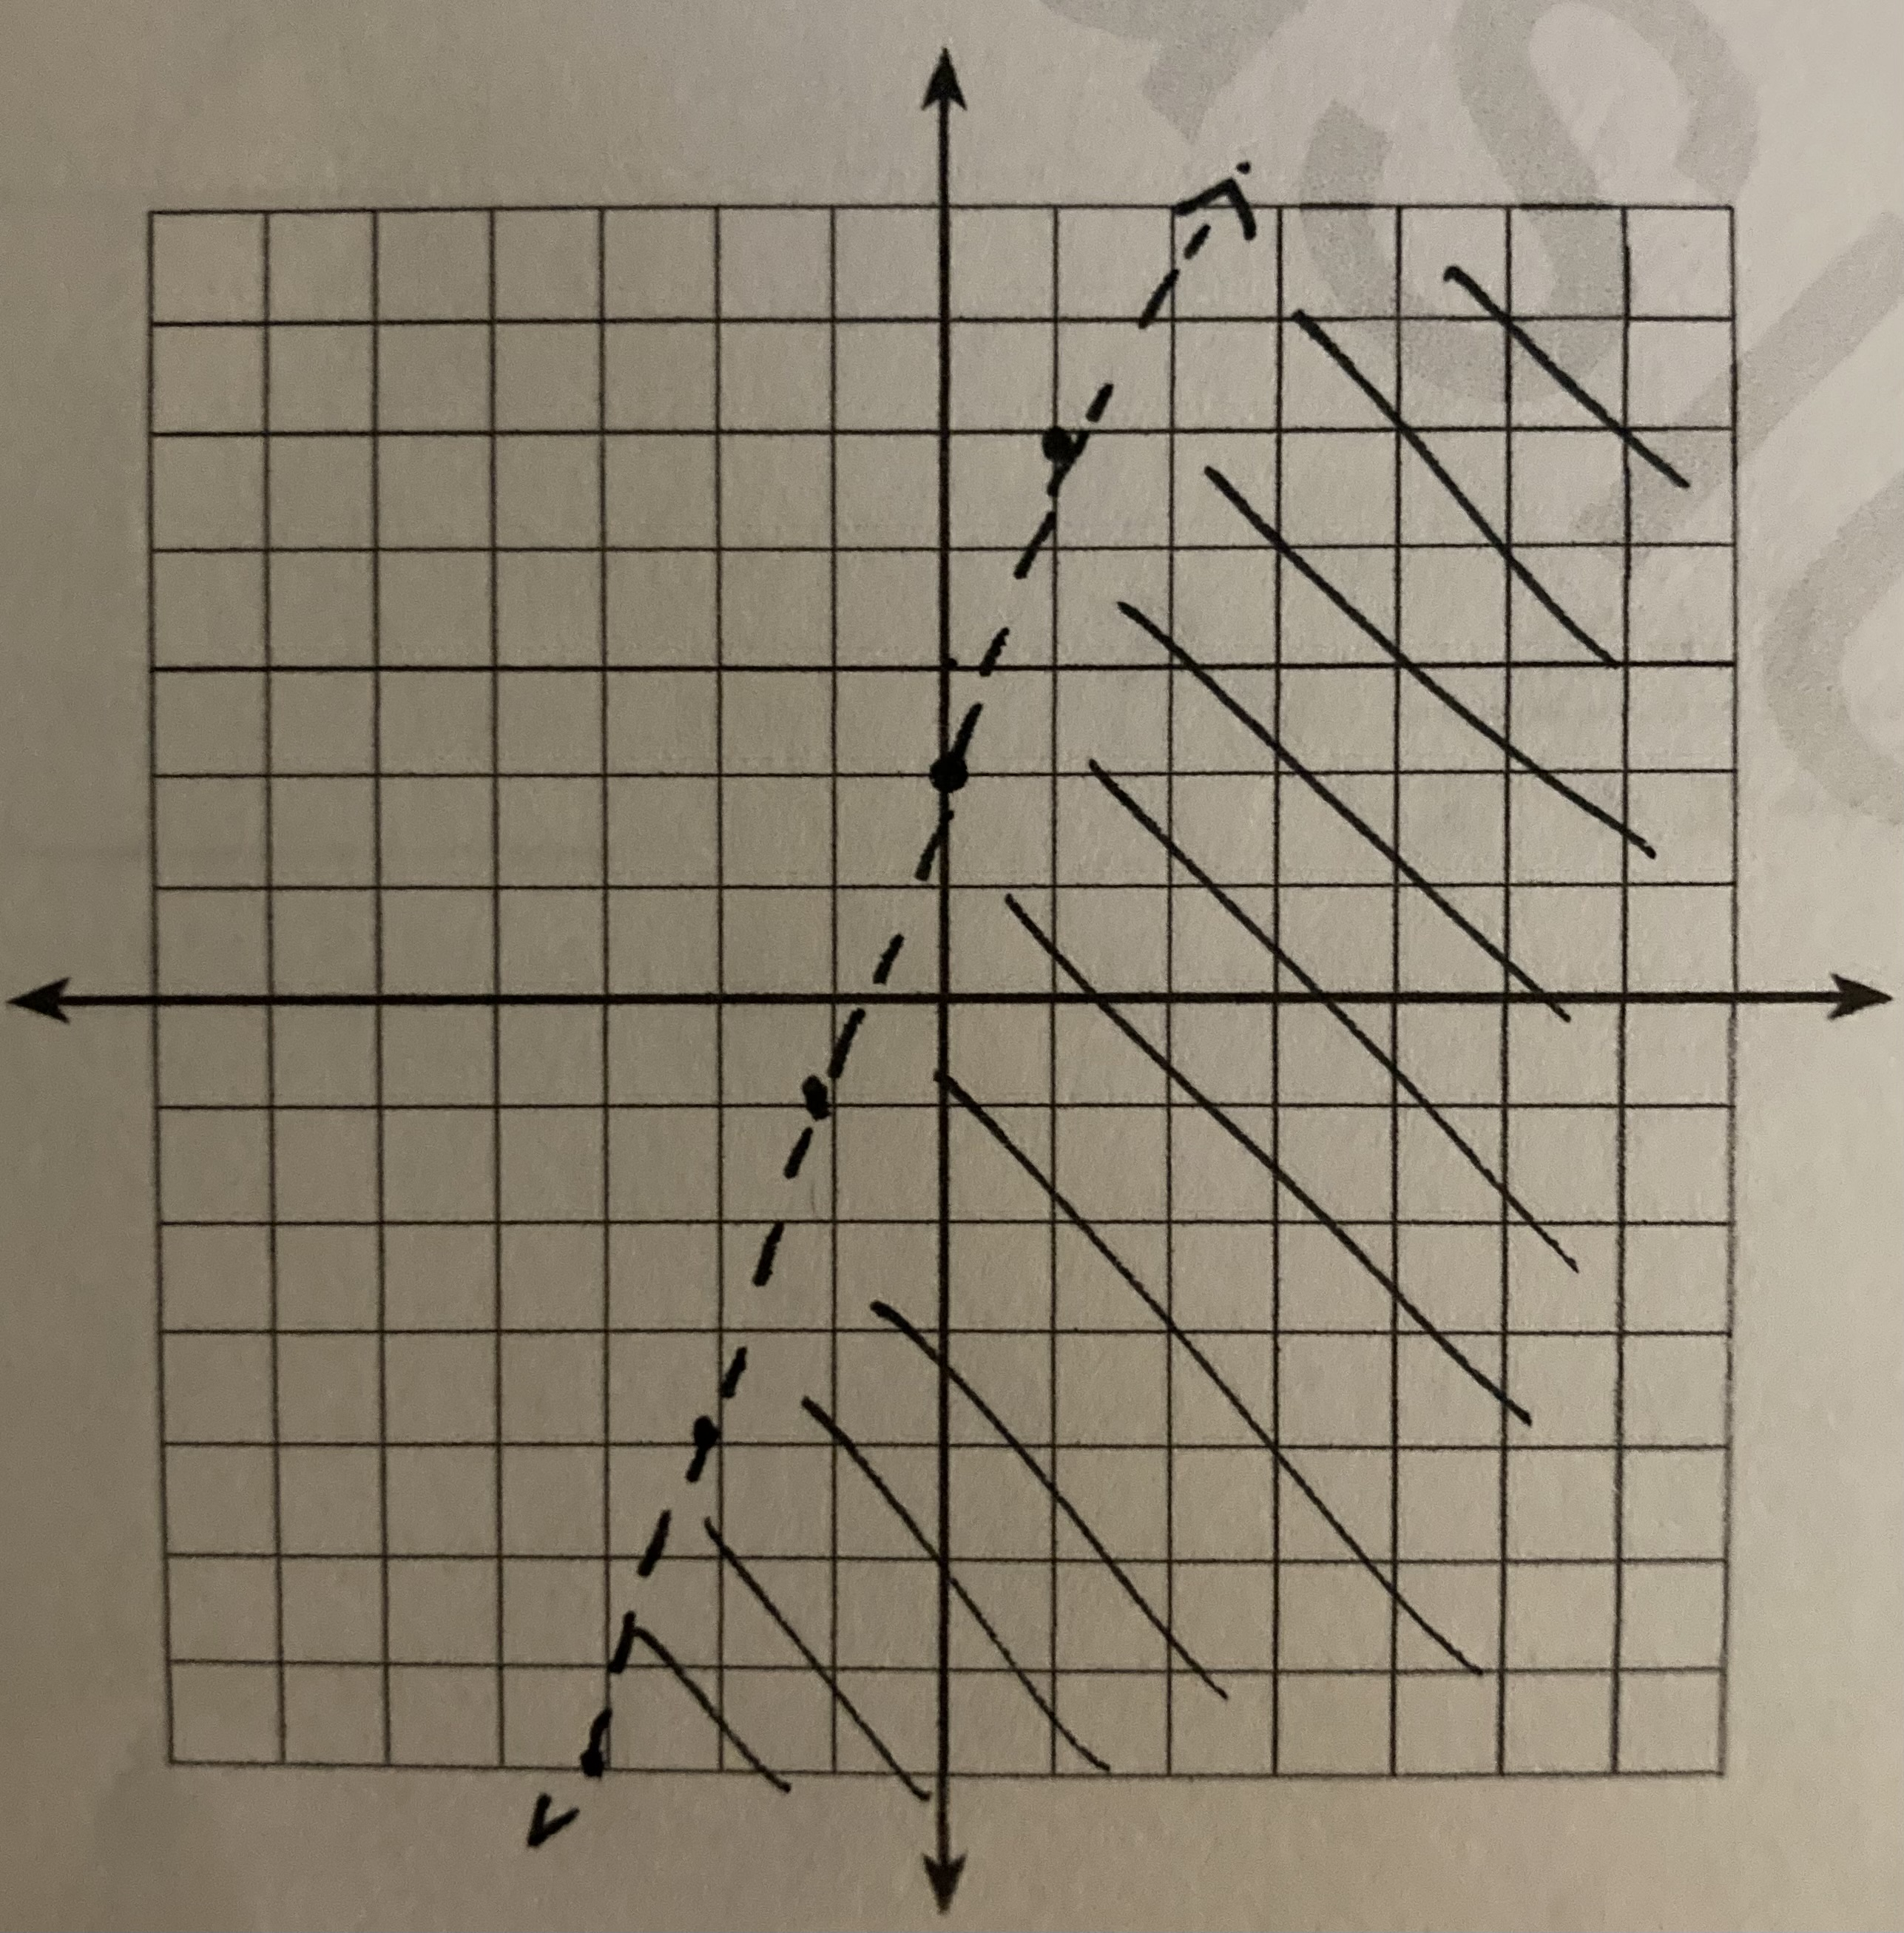
\includegraphics[width = 0.5 \textwidth]{67}
\end{center}
\end{enumerate}
today I will be proving the p-series test using the Cauchy Condensation test.
\begin{tcolorbox}
\begin{proof}
Let \( p > 1 \) and define the p-series as the following
\[ \sum_{n=1}^{\infty} \frac{1}{n^p}. \] 
Note that \( b_n = 1/n^p \) is decreasing and \( b_n \geq 0 \). We can use the Cauchy condensation test to prove the analogous series
\[ \sum_{n=1}^{\infty} 2^n \Big( \frac{1}{2^{n}} \Big)^p. \]
Since \( p > 1 \), this is equivalent to 
\[ \sum_{n=1}^{\infty} 2^n \Big(\frac{1}{2^n} \Big)^{p-1} = \sum_{n=1}^{\infty} \Big( \frac{1}{2^p}\Big)^n.\]
But notice that this is a \textit{geometric series} since \( p > 1 \) and \( |r| = 1/2^p < 1 \). Hence, the p-series converges.

\end{proof}
\end{tcolorbox}

Suppose we try and prove 
\[ \vec{F} = m \vec{a} = m \frac{d \vec{v}}{dt} = \frac{d}{dt}[m\vec{v}] = \frac{d\vec{p}}{dt}. \]

\begin{align*}
    |x - y |&= |x - x_n + x_n - y | \\
            &\leq |x - x_n| + |x_n -y| \\
            &< \frac{\epsilon}{2} + \frac{\epsilon}{2} \\
            &= \epsilon.
\end{align*}
Hence, the uniqueness of limits is proven. I like writing latex because the typesetting is very beautiful.  
This is to show how fast this auto preview is at compiling latex docs. 
I can say that I will only be using this when solving exercises for textbooks. 
Absolute convergence
\begin{align*}
    |t_n - t_m |&= \Big| \sum_{k=m+1}^{n} a_k  \Big|   \\
                &\leq \sum_{k=m+1}^{n} |a_k| \\ 
                &< \epsilon.
\end{align*}

Prove that \( \sup (A + B ) = \sup A + \sup B \).

\begin{tcolorbox}
    \begin{proof}
    By the Axiom of Completeness, the sets \( A,B \) are non empty and \textit{bounded above}. Hence, \( \sup A, \sup B \) exists and hence \( \sup ( A + B )\) exists.  Our goal is to show that \( \sup (A + B) \leq \sup A + \sup B \) and \( \sup ( A + B ) \geq \sup A + \sup B \). 

    Our first step is to show that \( \sup (A+B) \leq \sup A + \sup B \). Let \( a + b \in A + B \). By definition of \( \sup (A+B)\), we have that \( a + b \leq \sup (A+B)\). Suppose we add \( a \in A \) to both sides of this inequality. Hence, we have 
    \[ b \leq \sup (A +B ) - a.\]
    Since \( b \leq \sup B \) for all \( b \in B \), we have that 
    \[ \sup B \leq \sup (A+B) - a. \]
    Hence, we have 
    \[ a \leq \sup (A+B) - \sup B. \]
    Again, we have \( a \leq \sup A \) for all \( a \in A \). Hence, 
    \[ \sup A \leq \sup (A+B) - \sup B. \]
    Hence, 
    \[ \sup A + \sup B \leq \sup (A+B)\]  

    Now to show that \( \sup A + \sup B \geq \sup (A +B )\). By lemma 1.3.8, let \( \epsilon > 0 \). There exist \( \alpha \in A \) and \( \beta \in B \) such that 
    \begin{align*}
        \sup A - \frac{\epsilon}{2} &\leq \alpha \\
        \sup B - \frac{\epsilon}{2} &\leq \beta.  
    \end{align*}
    Adding these two inequalities together, we have
    \[ ( \sup A + \sup B ) - \epsilon \leq \alpha + \beta \]
    Since \( \epsilon > 0 \) is arbitrary, we have that \( \sup (A +B ) \geq \sup A + \sup B\).
    \end{proof} 
\end{tcolorbox}


Suppose we have a sequence \( (a_n) \) such that \( (a_n) \to 0 \) and we have a bounded sequence \( (b_n)\). Show that \( (a_n b_n ) \to 0 \). 
\begin{tcolorbox}
    \begin{proof}
    Let \( \epsilon > 0 \). Choose \( N \in \N \). Assume \( n \geq N \) and for some \( M > 0 \), we have 
    \begin{align*}
        |a_nb_n - 0 |&= | a_n b_n |  \\
                     &= |a_n| |b_n| \\
                     &< \frac{\epsilon}{M}\cdot M  \tag{\((b_n)\) is bounded }\\
                     &= \epsilon.
    \end{align*}
    Hence, \( (a_nb_n) \to 0 \). 
    \end{proof}
\end{tcolorbox}

Assume \( (x_n) \to x \). Show that \( \sqrt{x_n} \to \sqrt{x}\) where \( x_n \geq 0 \) for all \( n \in \N \). 
\begin{tcolorbox}
    \begin{proof}
    Let \( \epsilon > 0 \). Then 
    \begin{align*}
        |\sqrt{x_n} - \sqrt{x}|&= \Big| \frac{x_n - x}{\sqrt{x_n} + \sqrt{x}}\Big| \\
                               &= \frac{ |x_n - x|}{|\sqrt{x_n} + \sqrt{x}|} \\
                               &= 
    \end{align*}
    \end{proof}
\end{tcolorbox}







\end{document}
